%\documentclass[acmtog]{formats/acmart} 
\documentclass[acmtog]{acmart}
\makeatletter
\let\@authorsaddresses\@empty
\makeatother

%\documentclass[10pt, format=manuscript,nonacm]{acmart}

%\documentclass[acmtog,anonymous,review]{acmart}

\usepackage{soul}
\usepackage{booktabs} % For formal tables
\citestyle{acmauthoryear}
\setcitestyle{square}
\usepackage{ifthen}
\usepackage{enumitem}
\usepackage{algorithm}
%\usepackage{algorithmicx}
%\usepackage{algcompatible}
\usepackage[noend]{algpseudocode}
%\usepackage{algorithm2e}
\usepackage{float}
\usepackage{syntax}
\usepackage{amsfonts}
\let\Bbbk\relax
\usepackage{listings}
\usepackage{fancyvrb}
\usepackage{wrapfig}
\usepackage{graphicx}
\usepackage{subfigure}
\usepackage{xspace}
\usepackage{colortbl}
\usepackage{gensymb}
\usepackage{verbatim}
\usepackage{colortbl}
\usepackage{booktabs}
\usepackage{multirow}
\usepackage{cleveref}
\usepackage{pifont}
\usepackage{circledsteps}



%\lstset{style=mystyle}
\newcommand{\etal}{et al.}
\newcommand\TODO[1]{{\color{red} A: #1}}
\newcommand{\yuexin}[1]{{\color{blue} YX: #1}}
\newcommand{\ZY}[1]{{\color{cyan} ZY: #1}}
\newcommand{\manyi}[1]{{\color{brown} MY: #1}}
\newcommand{\haoran}[1]{{\color{olive} HR: #1}}
\newcommand{\yiteng}[1]{{\color{red} YT: #1}}
\newcommand{\yiming}[1]{{\color{orange} YM: #1}}
\newcommand{\changhe}[1]{{\color{orange} CH: #1}}


\usepackage{amsthm,amsmath,amssymb}
\usepackage{mathrsfs}
\usepackage[normalem]{ulem}
\begin{document}
\settopmatter{printacmref=false}
\setcopyright{none}
\renewcommand\footnotetextcopyrightpermission[1]{}
\pagestyle{empty} 

%\setcopyright{acmlicensed}
%\acmJournal{TOG}
%\acmYear{XXX} \acmVolume{XX} \acmNumber{XX} \acmArticle{XX} \acmMonth{XX} %\acmPrice{15.00}\acmDOI{10.1145/3618324}
\title{SymBridge: A Human-in-the-Loop Cyber-Physical Interactive System for Adaptive Human-Robot Symbiosis}


\author{Haoran Chen}
\authornote{Joint first authors.}
\affiliation{%
  \institution{Shandong University}
  \country{China}
}
\author{Yiteng Xu}
\authornotemark[1]
\affiliation{%
  \institution{ShanghaiTech University}
  \country{China}
}
\author{Yiming Ren, Yaoqin Ye}
\affiliation{%
  \institution{ShanghaiTech University}
  \country{China}
}

\author{Xinran Li, Ning Ding, Yuxuan Wu, Yaoze Liu}
\affiliation{%
  \institution{Shandong University}
  \country{China}
}

\author{Peishan Cong, Ziyi Wang, Bushi Liu, Yuhan Chen}
\affiliation{%
  \institution{ShanghaiTech University}
  \country{China}
}
%\author{Ziyi Wang}
%\affiliation{%
%  \institution{ShanghaiTech University}
%}
%\author{Bushi Liu}
%\affiliation{%
%  \institution{ShanghaiTech University}
%}
%\author{Yuhan Chen}
%\affiliation{%
%  \institution{ShanghaiTech University}
%}
\author{Zhiyang Dou}
\affiliation{%
  \institution{The University of Hong Kong}
  \country{China}
}
\author{Xiaokun Leng}
\affiliation{%
  \institution{LEJU(Shenzhen) Robotics Co., Ltd}
  \country{China}
}
\author{Manyi Li}
\authornote{Corresponding authors.}
\affiliation{%
  \institution{Shandong University}
  \country{China}
}
\author{Yuexin Ma}
\authornotemark[2]
\affiliation{%
  \institution{ShanghaiTech University}
  \country{China}
}
\author{Changhe Tu}
\affiliation{%
  \institution{Shandong University}
  \country{China}
}

\begin{abstract}
The development of intelligent robots seeks to seamlessly integrate them into the human world, providing assistance and companionship in daily life and work, with the ultimate goal of achieving human-robot symbiosis. This requires robots with intelligent interaction abilities to work naturally and effectively with humans.
However, current robotic simulators fail to support real human participation, limiting their ability to provide authentic interaction experiences and gather valuable human feedback essential for enhancing robotic capabilities.
In this paper, we introduce \textbf{SymBridge}, the first human-in-the-loop cyber-physical interactive system designed to enable the safe and efficient development, evaluation, and optimization of human-robot interaction methods. Specifically, we employ augmented reality technology to enable real humans to interact with virtual robots in physical environments, creating an authentic interactive experience. Building on this, we propose a novel robotic interaction model that generates responsive, precise robot actions in real time through continuous human behavior observation. The model incorporates multi-resolution human motion features and environmental affordances, ensuring contextually adaptive robotic responses. Additionally, SymBridge enables continuous robot learning by collecting human feedback and dynamically adapting the robotic interaction model. 
By leveraging a carefully designed system architecture and modules, \textit{SymBridge} builds a bridge between humans and robots, as well as between cyber and physical spaces, providing a natural and realistic online interaction experience while facilitating the continuous evolution of robotic intelligence. Extensive experiments, user studies, and real robot testing demonstrate the system's promising performance and highlight its potential to significantly advance research on human-robot symbiosis.
\end{abstract}


%\ccsdesc[500]{Computing methodologies~Shape modeling}
%\ccsdesc[300]{Computing methodologies~Graphics systems and interfaces}

%\acmJournal{TOG}

\keywords{Human-robot Interaction, Augmented Reality, Real-time Motion Generation}

\begin{teaserfigure}
%\vspace{-5pt}
  \includegraphics[width=1.0\linewidth]{images/teaser.png}
	\vspace{-15pt}
\caption {The SymBridge system enables natural real human-virtual robot interaction via an AR interface, supporting diverse actions like high-fives, pushes, and waves. Its interactive model improves continuously through human feedback and can eventually deploy to real robots for real-world use. The left image demonstrates SymBridge’s cyber-physical interaction with diverse interaction categories, and the right displays real-world human-robot interaction.}
%Concurrently, humans gradually develop a deeper understanding and trust in the robot. Ultimately, SymbioSim fosters bidirectional learning and adaptation, with the potential to promote human-robot symbiosis.}
  \label{fig:teaser}    
\end{teaserfigure}

%\input{macros}
\maketitle


\section{Introduction}
\label{sec:intro}

With rapid advancements in robotics and artificial intelligence, robots are moving from industrial settings into everyday human environments~\cite{lecun2022path,gonzalez2021service}, showing promise in areas like daily service, home care, and healthcare. To achieve the vision of human-robot symbiosis, the most challenging issue is how to enable robots to interact and collaborate with humans as naturally and efficiently as possible in daily life.%while ensuring safety and privacy protection.
%The ultimate goal is not just to handle repetitive or dangerous tasks, but to work alongside humans to improve efficiency and quality of life—achieving human-robot symbiosis. 
%Realizing this vision requires harmonious and effective communication and interaction between humans and robots, encompassing both verbal and behavioral exchanges. 
%While large language models~\cite{roumeliotis2023chatgpt,touvron2023llama} have made language-based communication easier, major challenges remain in behavioral interaction~\cite{safavi2024emerging}, which involves empowering robots to perceive and interpret human intentions through observation and reasoning, and to adapt their own actions accordingly—fostering seamless, natural collaboration in shared environments.


To support the development and evaluation of intelligent robotic algorithms, over the past few decades, many robotic simulators~\cite{makoviychuk2021isaac, todorov2012mujoco,igibson, nasiriany2024robocasa} have emerged and been widely used. They are well-suited for tasks such as robotic navigation, manipulation, and control within predefined digital environments containing static objects. However, they struggle to support human-robot interaction (HRI), as modeling human behavior—especially the complex, dynamic, and closed-loop interactive behavior—is extremely challenging. To bridge this gap, recent work~\cite{HumanTHOR, liu2024collabsphere} has shifted toward incorporating real humans into HRI simulations. However, these systems still have limitations: humans generally control virtual avatars through keyboards or VR interfaces to collaborate with simulated robots. The focus is on completing tasks that do not involve close physical interaction. So far, there still lacks 3D physical interaction, preventing truly realistic and immersive human-robot behavioral exchange. %This setup lacks 3D physical interaction, preventing truly realistic and immersive human-robot behavioral exchange.

%Just as humans usually learn and grow through practice, robots are required to gain knowledge and skills through continuous real-world interactions, progressively enhancing their intelligence. Nevertheless, due to concerns about efficiency, cost, and safety, most current research on embodied intelligence avoids direct use of physical robots, relying instead on physical~\cite{makoviychuk2021isaac, todorov2012mujoco} or robotic simulators~\cite{igibson, nasiriany2024robocasa}. These simulators are well-suited for tasks such as navigation, manipulation, and control within predefined digital environments containing static objects. However, they struggle to support human-robot interaction (HRI), as modeling human behavior—especially modeling complex, dynamic, and closed-loop interactive behavior—is extremely challenging.
%Recent efforts~\cite{HumanTHOR, liu2024collabsphere} have begun to address the integration of humans into robotic simulation platforms, these approaches typically depend on keyboard or VR-based control of virtual avatars for task-level collaboration with virtual robots. 
%However, humans cannot interact directly with robots in a physical environment, limiting the emergence of authentic interactive behaviors. More importantly, robots are unable to observe real human actions, making it difficult to develop and evaluate intelligent interactive models for robots.

%To enable seamless human-robot coexistence through natural and trustworthy interaction, it is essential to develop human-in-the-loop interactive platforms. Such system would allow real humans to engage in authentic interactions and provide real-time feedback during interaction with robots, ultimately driving the evolution of robotic interactive capabilities toward true symbiosis.
% \begin{haoran}
To address this gap, our system aims to enable real-time and realistic human–robot interaction through AR. AR allows humans to interact directly with virtual robots, and through repeated interactions, users develop familiarity with robot behaviors. Over time, the system collects human feedback that continuously improves robot motion generation. Together, these elements represent a first step toward achieving human–robot symbiosis.
% \end{haoran}

To facilitate the development, evaluation, and evolution %iteration
of HRI algorithms—ultimately enabling intelligent robots to provide direct services to humans—a simulation system supporting authentic HRI experiences is crucial. However, this presents significant challenges: 
%\textbf{1)} How can we accurately represent realistic human behavior? 
\textbf{1)} How to involve real humans interacting with virtual robots in physical space for authentic interaction experience? \textbf{2)} How to drive virtual robots to respond to human actions in real-time, achieving natural and seamless interactive behaviors? \textbf{3)} How to enable continuous algorithmic self-improvement through ongoing interaction, ultimately creating intelligent robots that meet human expectations?

In this paper, we present SymBridge, a pioneering human-in-the-loop robotic interaction system designed for achieving human-robot symbiosis, as Fig.~\ref{fig:teaser} shows. %First, in SymBridge, we employ a LiDAR-based motion capture system to digitize 3D human motions in real time. This approach not only captures precise movement data but also offers inherent privacy preservation by avoiding the collection of any appearance textures or identifiable visual features. Second, we utilize the augmented reality (AR) technology to connect the real human and virtual robot by rendering robot in physical environment by AR glass to provide authentic interactive experience for users. Third, we propose an efficient and effective robotic interaction model to drive robots naturally responds to human actions for completing diverse interactive behaviors. Unlike other offline motion generation methods~\cite{xu2023interdiff,xu2024regennet}, our interaction model could support real-time, online robot action generation. This capability enables the robot to dynamically adapt to rapid changes in human behavior. Moreover, our method learns hierarchical human behavior features and leverages affordance prediction to guide more precise interaction actions, ultimately achieving a natural and smooth interaction experience.  Finally, SymBridge can automatically collect human feedback throughout the interaction process and use the recorded data to fine-tune the robots' capability, enabling the robot's behaviors to progressively adapt to user preferences, creating a "better with use" robotic evolution mechanism. By this, SymBridge can significantly reduce the costs and risks of developing intelligent interaction models for robots.
%SymBridge integrates three key innovations to address above three challenges. 
SymBridge innovatively addresses the above challenges with the following key characteristics: 

\noindent\textit{\textbf{1) Realistic Interaction Interface}}: SymBridge simulates robot perception with a LiDAR-based motion capture system and presents robot reactions through augmented reality (AR) technology. The LiDAR-based MoCap module implements real-time 3D human motion digitization while robust to varying lighting conditions and ensuring privacy-preserving. The AR interface bridges the physical and virtual realms by rendering virtual robots into the user’s environment via AR glasses, creating an immersive, authentic interactive experience that seamlessly blends human and robotic actions. %In addition, to enable accurate robot perception of 3D human movements, SymBridge leverages a precise LiDAR-based motion capture system for real-time 3D human motion digitization. This solution is robust to varying lighting conditions while ensuring ensures privacy-preserving.

\noindent\textit{\textbf{2) Real-Time Robotic Interaction Model}}:
Unlike offline motion generation methods, SymBridge's interaction model enables online, real-time robot action generation. Its key innovation lies in the synergistic integration of spatial reasoning and temporal understanding. Specifically, it fuses an Affordance Predictor for fine-grained spatial awareness with a Multi-Resolution Human Feature (MRHF) Learner that captures deep temporal context. This holistic approach, distinct from prior work (e.g., JRT~\cite{xu2023joint}, ReGenNet~\cite{xu2024regennet}) that often addresses these aspects separately, allows the model to generate responses that are simultaneously contextually and socially-aware, adapting instantly to rapid changes in human behavior.
% Unlike offline motion generation methods (e.g.,~\cite{xu2023interdiff,xu2024regennet}), SymBridge’s interaction model enables online, real-time robot action generation. By dynamically analyzing hierarchical human behavior features and leveraging affordance prediction, the system generates precise, context-aware robotic responses that adapt instantly to rapid changes in human behavior, ensuring more natural and smooth interactions compared to recent relevant approaches.

\noindent\textit{\textbf{3) Feedback-Driven Adaptation Mechanism}}:
SymBridge continuously collects human feedback during interactions and uses this data to iteratively fine-tune the robot’s capabilities. This creates a "better with use" evolution mechanism, where the robot’s behavior progressively aligns with user preferences, significantly simplifying and boosting the improvement of robotic intelligence.

\noindent Together, these components establish SymBridge as a pioneering system for human-robot interaction, %where privacy, adaptability, and user-centric evolution converge to enable safe, efficient, and intuitive interaction paradigms.
which enables immersive, intuitive, and efficient interaction paradigms.
As a dual bridge between humans and robots and physical and virtual worlds, SymBridge accelerates the realization of human-robot symbiosis, with the potential to pave the way for collaborative ecosystems where robots and humans evolve in tandem.



%In SymBridge, users interact with virtual robots through augmented reality (AR) glasses. As Fig.~\ref{fig:teaser} shows, the platform captures human motions as the robot's perception and presents the virtual robot's reaction to the user from first-person and third-person perspectives. It can automatically collect human feedback throughout the interaction process and use the recorded data to fine-tune the robots' capability, enabling the robot's behaviors to progressively adapt to user preferences, creating a "better with use" robotic system. By this, SymBridge can significantly reduce the costs and risks of developing intelligent interaction models for robots. Simultaneously, users develop a deeper understanding of the robot's intentions and refine their interaction strategies, fostering greater trust and enabling the robot’s seamless integration into daily life. As a dual bridge between humans and robots and physical and virtual worlds, SymBridge accelerates the realization of human-robot symbiosis, with the potential to pave the way for collaborative ecosystems where robots and humans evolve in tandem.

%In particular, to facilitate the validation of SymBridge platform, we provide a novel and effective method for humanoid robot motion generation, enabling the robot to respond promptly to human actions and successfully complete interaction tasks. Unlike other offline motion generation methods~\cite{xu2023interdiff,xu2024regennet}, our robotic interaction model could support real-time, online robot action generation. This capability enables the robot to dynamically adapt to rapid changes in human behavior. Furthermore, our method hierarchically models observed human behavior and leverages affordance prediction to guide more precise interaction actions, ultimately achieving a natural and smooth interaction experience.  


To demonstrate the effectiveness of our solution, we have developed a comprehensive evaluation methodology and benchmark for human-robot interaction, complementing both quantitative and qualitative assessments of the algorithmic components within our system.
Further, we evaluate the efficiency and quality performance of our system when facilitating human users to interact with the virtual robot. 
A user empirical test with 50 participants confirms that human users are satisfied with the realistic and real-time interaction experience via our system. We also deploy the generated virtual robot reactions to a real humanoid robot to examine the realism and fidelity of the robot movements presented with our system. Additionally, by fine-tuning our model with user feedback data, we demonstrate continuous performance improvement, proving our system's capability to enhance robotic interaction models through ongoing interactive data collection. 

%We conduct comprehensive experiments to validate the effectiveness and practicality of the SymBridge platform. First, through both qualitative and quantitative evaluations, we validate the superior performance of our robotic interaction model compared to other alternative solutions.
%Second, we evaluate the time and quality performance of the platform when facilitating human users to interact with the virtual robot. 
%A user empirical test with 50 participants indicates that human users are satisfied with the realistic and real-time interaction experience. We also deploy the virtual robot reactions to a real humanoid robot to examine the realism and fidelity of the interactions presented with our platform. Third, we show the performance improvement of the robotic interaction model after fine-tuning it with more positive and negative interaction data, demonstrating that our platform can assist model's improvement by collecting authentic human-robot interaction data and user feedback. 

%Our contributions are summarized as follows:
%\begin{itemize}
%\item We introduce SymBridge, the first human-in-the-loop cyber-physical system, designed to enable real-time, realistic interactions between human users and virtual robots, and also support feedback-driven adaptation of robotic models.
%\item We propose a novel robotic interaction model, supporting online precise humanoid robot motion generation for versatile human-robot interactions.
%\item We conduct comprehensive evaluations as well as user empirical test and real robot test, to validate the effectiveness and practicality of our system and internal modules.
%\end{itemize}


\input{sections/2-relatedWork}

\begin{figure*}
\centering
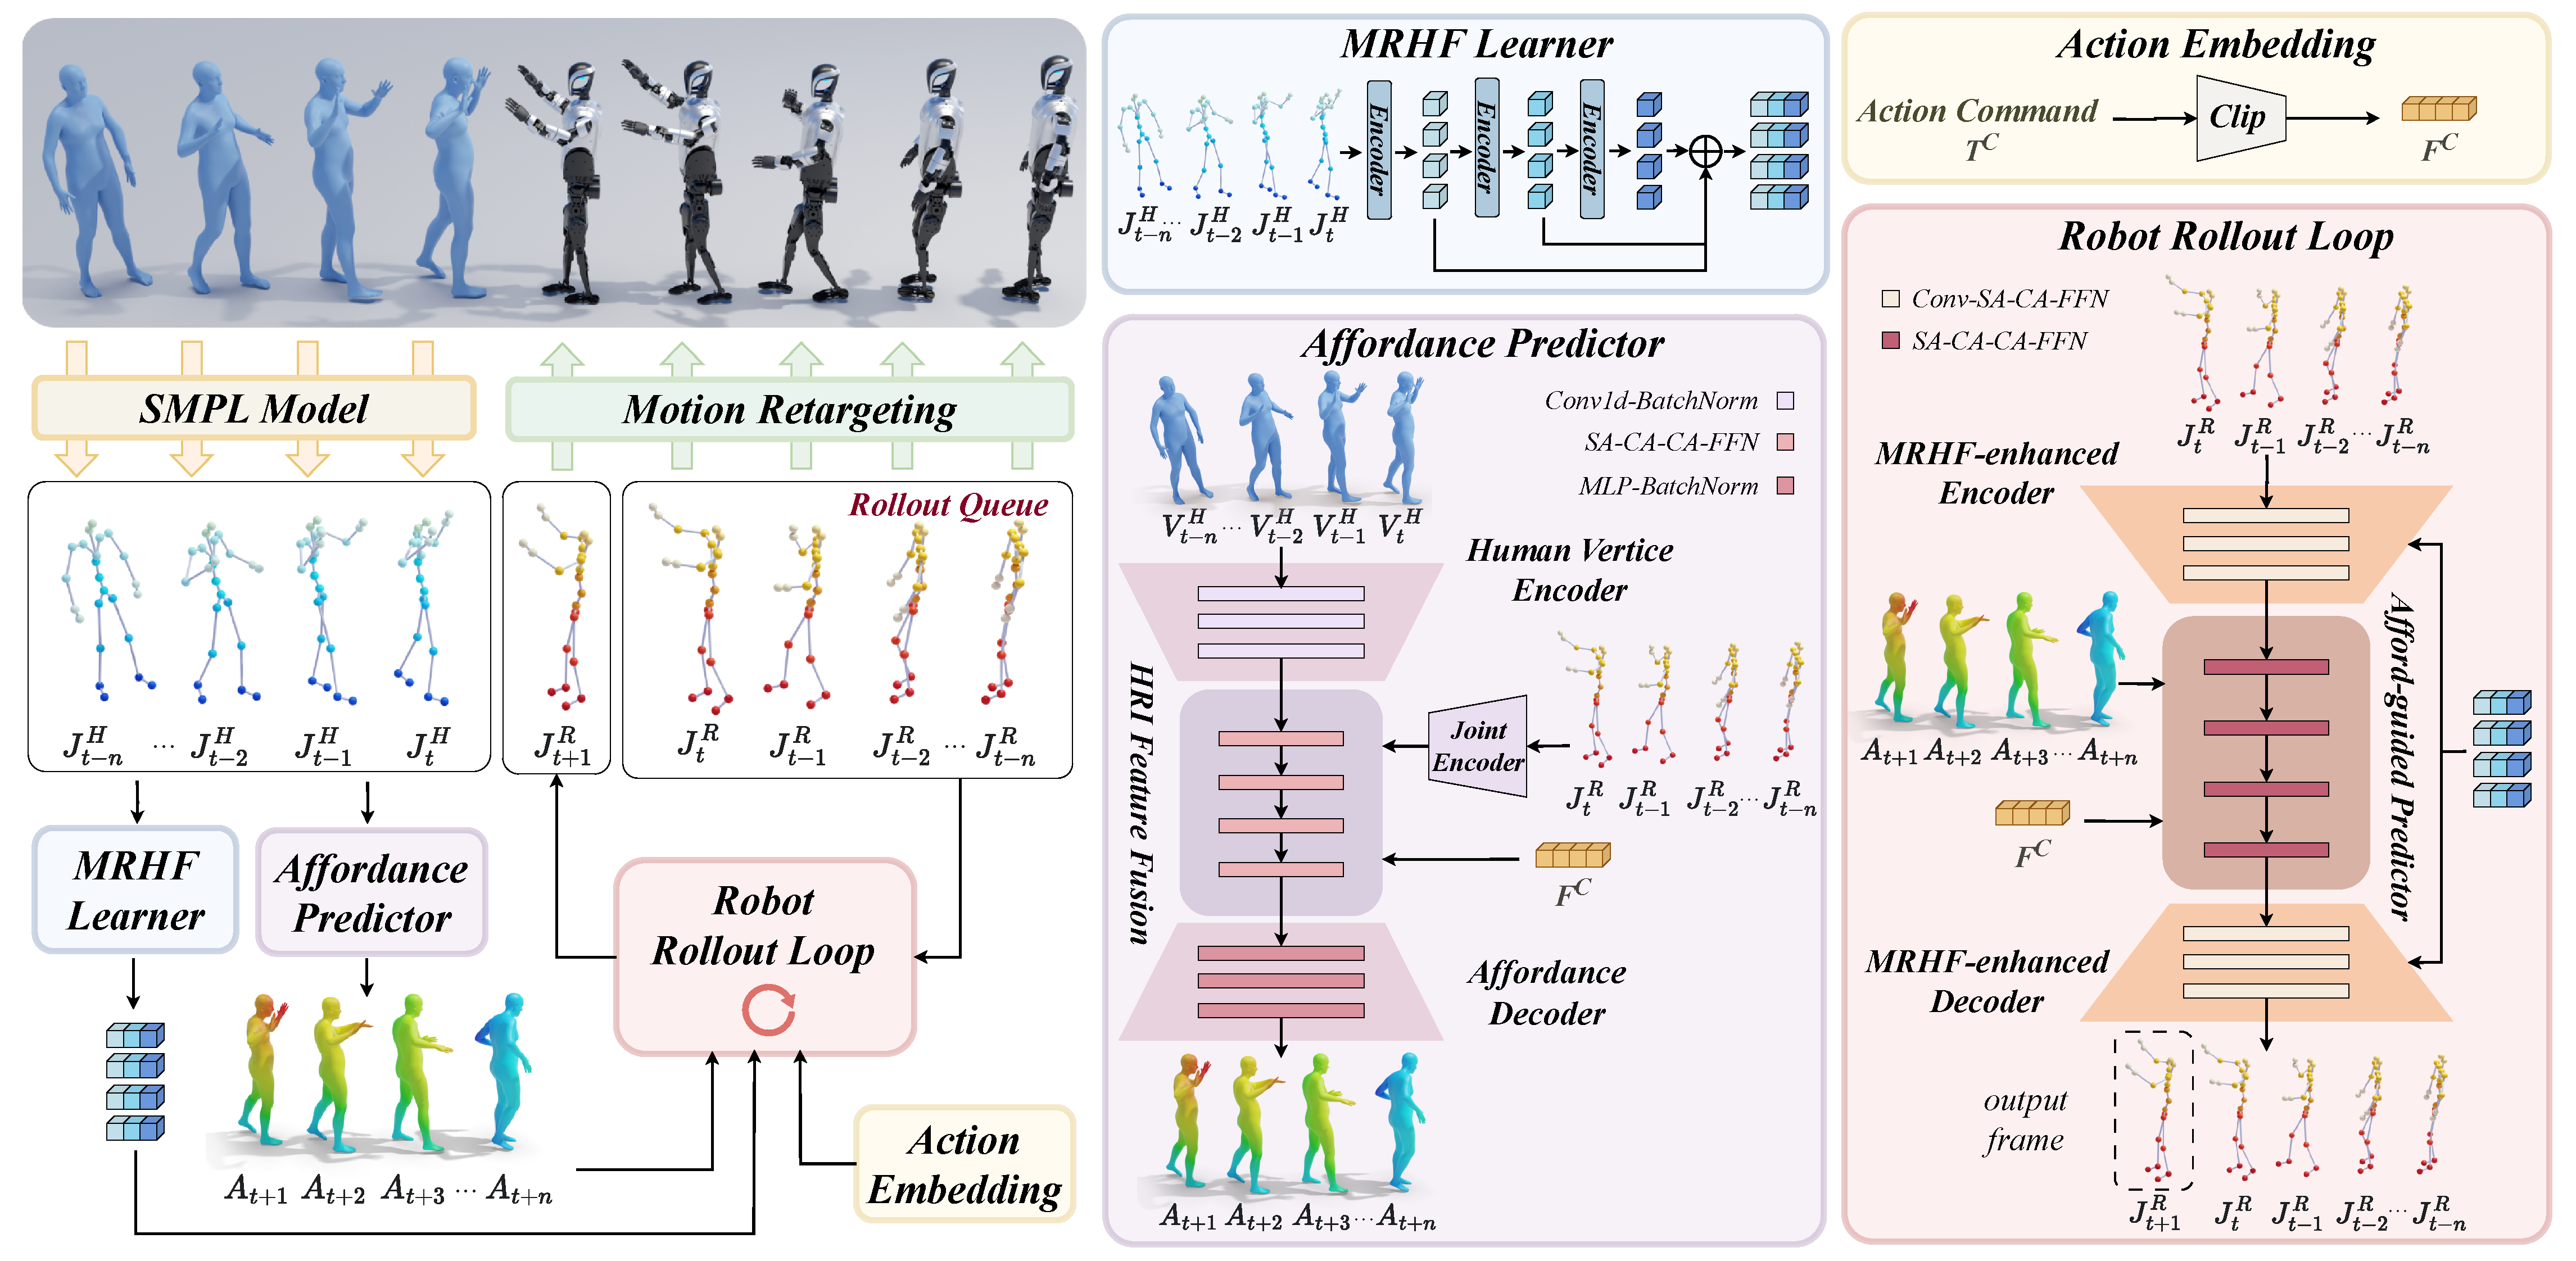
\includegraphics[width=1\linewidth]{images/intermodel-mainv5.pdf}
\vspace{-20pt}
\caption{Overall pipeline of our Robotic Interaction Model. The model ingests text action commands, historical robot joints, observed human joints and SMPL mesh vertices, and processes them through four tightly coupled modules. The Affordance Predictor explicitly estimates dense end-effector–vertex spatial fields to enable dexterous, socially-appropriate contact reasoning; the Multi-Resolution Human Feature (MRHF) Learner fuses hierarchical temporal cues to boost situational awareness; the Robot Rollout Loop leverages these affordance and human features to iteratively generate coherent, context-adaptive joint trajectories for real-time responsiveness; and finally, the Motion Retargeting module maps each predicted skeleton frame to robot-specific angle axis.}
\label{fig:interactiveModel}
\vspace{-10pt}
\end{figure*}
\section{Design Goals}

Towards the human-robot symbiosis, our primary purpose is to develop a human-in-the-loop system that supports the versatile interactions between humans and robots, such as hand-shaking, hugging, etc. In this way, human users can easily obtain more experiences to get used to interacting with robots and returning their authentic feedback to improve robot skills to better facilitate human life. We decompose it into specific design goals as follows.

\noindent\textbf{D1. Simulate a realistic and real-time human-robot interaction experience.} To allow human users to interact with virtual robots, the system must capture human motion, produce a robot reaction, and present it to the user. More importantly, the whole pipeline should be realistic and real-time enough for the user to have an immersive experience like interacting in the real world.

\noindent\textbf{D2. Produce reasonable and plausible robot reactions regarding human behavior.} 
Humans may perform various actions during interactions. The fundamental capability of the system is to automatically determine the appropriate robot reaction based on human behavior to ensure a fluent human-robot interaction.

\noindent\textbf{D3. Facilitate human feedback collection for robot interaction skill enhancement.} Over the long-term interactions, humans and robots should mutually adapt to each other to achieve harmonious co-existence. It requires an efficient fine-tuning mechanism to continuously enhance the robot's interaction skills. Therefore, the system should facilitate the collection of human-robot interaction data with authentic human feedback and efficiently utilize the collected data to fine-tune robot interactions.

\section{Symbridge System}
\subsection{System Architecture}

The aforementioned design goals lead to our system architecture, as illustrated in Fig.~\ref{fig:system}. The core is the immersive human-robot interaction with our AR interface, where a human user can wear AR glasses to interact with the virtual robot in the real environment. It activates the two main capabilities of our system.


The \emph{human-robot interaction}, illustrated with the blue arrows in Fig.~\ref{fig:system}, aims to support the realistic and real-time interactions between humans and the virtual robot. First, the human behavior is continuously acquired as motion sequences by the motion capture module. Given the current frame and the cached historical frames of the captured human motion, we employ an interactive model to predict the next frames of the robot motion. The predicted robot motion is sent %to the physical simulation module, which leverages a physical humanoid controller to infer the physically feasible robot reactions that align with the predicted robot motion as much as possible. Finally, the simulated robot poses are transmitted 
to the applications running on the AR glasses to provide immersive interaction experiences. Our system also provides a third-person perspective by presenting the captured real human and rendered virtual robot on the same visual frame.

The \emph{model adaptation}, illustrated with the yellow arrows in Fig.~\ref{fig:system}, aims to enhance the robot's interaction skills by collecting and utilizing the human-in-the-loop interaction data. During the human-robot interaction through the AR interface, the human users may express their feedback, such as ratings on the quality of interaction experiences. Our system records the interaction process as well as the human feedback, and utilizes them to fine-tune the interactive model to adapt it to human preference. %After fine-tuning, the interactive model is updated to further assist the human-robot interactions. 

\subsection{Modules for Human-Robot Interaction}
\label{sec:mocap}
%To facilitate realistic and real-time human-robot interaction, the platform should capture human motions to mimic robot perception and present the robot reactions to the user. They can be considered as providing the input and processing the output of a pluggable \textbf{Robotic Interaction Model}, which will be introduced in Section~\ref{sec:interactivemodel}.

\noindent\textbf{Motion Capture.} To enable realistic and real-time human–robot interaction, the system requires accurate motion capture that approximates the robot’s perception. We employ an Ouster OS1-128 LiDAR sensor to acquire 3D point clouds of the human subject. This device provides high-precision depth information while inherently preserving user privacy by not capturing appearance textures. Moreover, it operates robustly under varying lighting conditions. In our setup, the LiDAR is positioned in front of the user, who can move within a range of 5–7 meters from the sensor.
Then, we employ the cutting-edge LiDAR-based framework LiveHPS++~\cite{ren2025livehps++}, which estimates pose parameters of human motions from scanned point clouds. More details are in supplementary material. %During the interactions, we set a 10FPS speed of the motion capture system due to the limit of the LiDAR device.

%\noindent\textbf{Interactive Model.} Given the human pose parameters from the motion capture module, we first convert them into joint positions of the human body skeleton with a forward kinematic algorithm. Then, for every frame, the interactive model takes historical and current human poses and robot poses, as well as the user's action command such as "handshake" as input, and outputs a sequence of the predicted \color{red}next \color{black} robot poses. All the input and output poses of the interactive model are represented as the joint positions of the skeletons, either of a human or a robot body, \color{red}for ...\color{black} After that, we further convert the output robot pose via an online inverse kinematics solver. [Why include these FK and IK? One can also ...]

%\noindent\textbf{Physical Simulation.} We employ the deep reinforcement learning technique presented in~\cite{luo2023perpetual} to control simulated robots in a physical simulation environment, i.e., IssacGym~\cite{makoviychuk2021isaac}. The objective is to achieve maximum alignment between predicted robot poses with the real robot poses (also as known as motion tracking for physical agents) while maintaining physical plausibility. Specifically, we train the xxx. During inference, to achieve our real-time purpose, \color{red}at each timestep, we \color{black}

\noindent\textbf{Robotic Interaction Model.} To enable robots to interact with humans naturally and smoothly, we have designed an efficient robot interaction model. This model uses motion-captured human movements as observational data to generate real-time motion responses, driving virtual robots to interact with real humans in 3D space. The technical approach is introduced in Section~\ref{sec:interactivemodel}.

\noindent\textbf{First-Person Perspective on AR Glasses.} We employ an AR device, i.e. PICO4 Ultra~\cite{PicoInteractive2022}, to visualize virtual robots from the first-person perspective. It communicates with the interactive model through TCP protocol to update the robot positions and poses. The virtual robot is seamlessly integrated into the real environment %backbround 
with photorealistic rendering.

\noindent\textbf{Third-Person Perspective on Screen.} To show the panoramic view of the interaction between the real human and the virtual robot, we set up an RGBD camera and calibrated its intrinsic and extrinsic parameters. After that, we render the virtual robot from the calibrated viewpoint and fuse it with the image captured by the camera based on their corresponding depth maps.

 %Addressing occlusion and multi-user scenarios remains an important direction for future work, which may involve sensor fusion, predictive modeling of partially observed human motion, and adaptive fail-safe mechanisms.

\subsection{Modules for Model Adaptation}

Model adaptation involves the collection of human-robot interaction records and human feedback, and utilizing them to effectively fine-tune the interactive model for robot skill enhancement.

\noindent\textbf{HRI Data and Feedback Collection.} Throughout the interactions process, we record the interaction data in different modalities, including the scanned point cloud and captured pose parameters of the human user, as well as the robot's pose parameters and skeleton keypoint positions. Meanwhile, users can provide feedback in various forms, such as direct ratings or detailed language descriptions of their interaction experience. 

%Additionally, implicit feedback can be captured through users' actions, which may reflect their comfort level, engagement, or preferences during the interaction. The collected feedback, combined with the recorded human-robot interaction data, forms comprehensive human-in-the-loop realistic data for fine-tuning the foundational interactive model.

\noindent\textbf{Model Fine-tuning.}
We classify the interaction data into positive and negative samples~\cite{zhu2025evolvinggrasp} based on the user ratings. Positive samples represent the cases that are well-received by users, while negative samples are those that users find unsatisfactory or unnatural. Our system supports a supervised learning paradigm to refine and adjust the interaction model by effective fine-tuning strategies. This allows the robot to better align with user needs and preferences. %Through this closed-loop feedback mechanism, the robot progressively improves its interaction quality, enabling more natural and efficient collaboration with humans.


\section{Robotic Interaction Model}
\label{sec:interactivemodel}
% \begin{figure*}
\centering
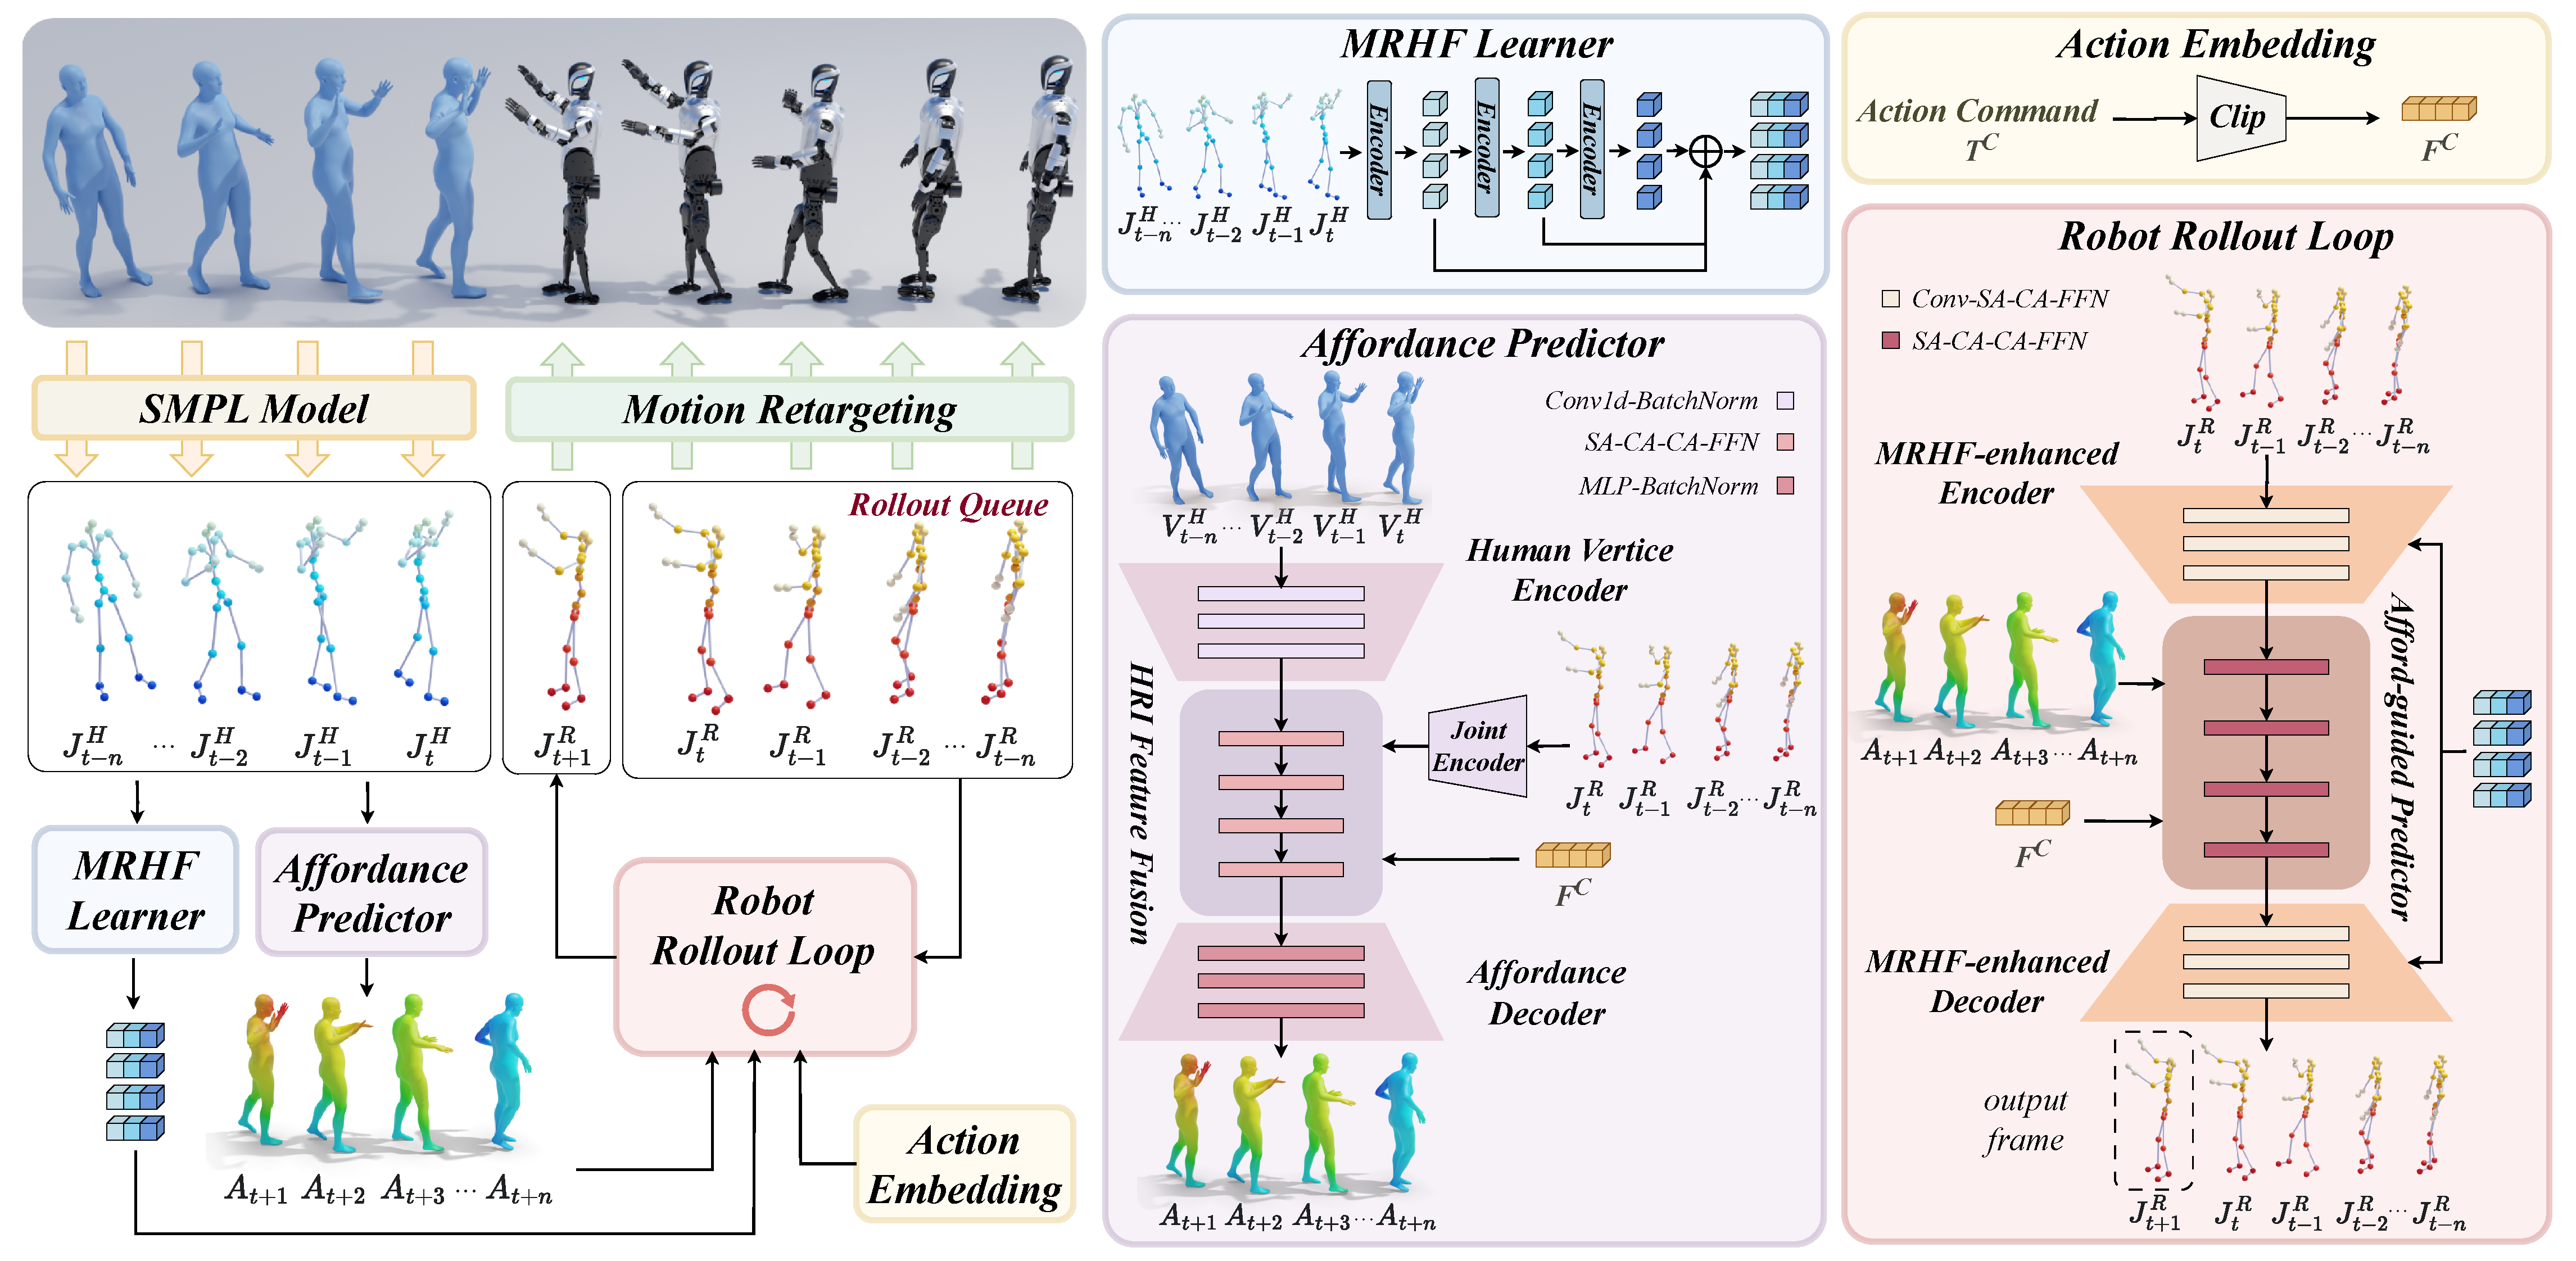
\includegraphics[width=1\linewidth]{images/intermodel-mainv5.pdf}
\vspace{-20pt}
\caption{Overall pipeline of our Robotic Interaction Model. The model ingests text action commands, historical robot joints, observed human joints and SMPL mesh vertices, and processes them through four tightly coupled modules. The Affordance Predictor explicitly estimates dense end-effector–vertex spatial fields to enable dexterous, socially-appropriate contact reasoning; the Multi-Resolution Human Feature (MRHF) Learner fuses hierarchical temporal cues to boost situational awareness; the Robot Rollout Loop leverages these affordance and human features to iteratively generate coherent, context-adaptive joint trajectories for real-time responsiveness; and finally, the Motion Retargeting module maps each predicted skeleton frame to robot-specific angle axis.}
\label{fig:interactiveModel}
\vspace{-10pt}
\end{figure*}

Real-time, context-aware motion generation remains a persistent challenge for human-robot interaction, especially in dynamic and contact-rich scenarios.
Existing approaches~\cite{wang2021multi,xu2024regennet,mueller2024massively} for interactive robot motion generation often fail to adequately address real-time responsiveness and realistic interaction dynamics. To address these challenges, we propose a novel Robotic Interaction Model capable of generating coherent and timely interactive motion sequences for humanoid robot with three main technical advances:

%\begin{itemize}
\noindent\textbf{1) Affordance Predictor} precisely captures fine-grained spatial and geometric relationships between robot end-effectors and the human body, which is crucial for guiding the generation of precise and socially-appropriate interactive actions.
\noindent \textbf{2) Multi-Resolution Human Feature (MRHF) Learner} integrates human behavioral features at multiple temporal scales, improving the understanding of human intentions.
\noindent \textbf{3) Robot Rollout Loop} enables real-time, coherent, and context-adaptive robot motion, ensuring both responsiveness and long-term stability. It provides a solid guarantee for smooth and realistic interactive experience of the system.
%\end{itemize}


\subsection{Model Input and Output}
Our model generates humanoid robot motions in an online fashion by conditioning on both human behavior and robot history. As shown in Fig.~\ref{fig:interactiveModel}, the model takes three inputs at each timestep.
\noindent\textbf{Textual Command ($T^C$)} is a user-specified action prompt such as \textit{``High-five''} or \textit{``Handshake''}, representing the intended interaction type. Our Action Embedding module uses a pre-trained CLIP~\cite{radford2021learning} text encoder to map it to a visual-aware feature $F^C$, which is then fused with motion features in downstream modules to guide context-aware motion generation.
\noindent\textbf{Historical Robot Motion ($J^{R}_{t-n\sim t}$)} is a sequence of past robot joint skeletons, stored in a rollout queue from timestep $t - n$ to $t$. \noindent\textbf{Human Motion Observation} includes human joint skeletons ($J^{H}_{t-n\sim t}$) and SMPL mesh vertices ($V^{H}_{t-n\sim t}$). Both are obtained by applying the SMPL model to the pose parameters \( P^{H}_{t-n\sim t} \) and translation parameters \( T^{H}_{t-n\sim t} \) from the motion capture mentioned in Section~\ref{sec:mocap}. 


The model outputs a future sequence of predicted robot skeletons $J^R_{t+1 \sim t+k}$. We then employ a \textbf{receding horizon strategy}: only the immediate next frame $J^R_{t+1}$ is executed, while the rest of the sequence is discarded. This approach is crucial for balancing long-term motion coherence with real-time responsiveness. Predicting a multi-frame sequence ensures that the generated motion is smooth and natural, guided by sequence-level supervision. Conversely, executing only the first frame enables the robot to immediately adapt to dynamic human behavior by re-planning at every timestep. This continuous cycle not only guarantees high responsiveness but also enhances robustness by mitigating the accumulation of prediction errors.

% The model outputs a future sequence of predicted robot skeletons $J^{R}_{t+1\sim t+k}$ for the consistency of predicted robot motion. However, \textbf{only the immediate next frame} $J^{R}_{t+1}$ is executed by robot, and the rest of the sequence is discarded to guarantee online generation.




%The frame-by-frame rollout strategy enables real-time interactivity by:
%\textbf{Responsiveness}: Adapting quickly to unexpected human actions.
%\textbf{Robustness}: Avoiding error accumulation from long-term predictions (unlike offline methods~\cite{mueller2024massively,wang2021multi,xu2024regennet}).
%\textbf{Coherence}: Maintaining fluid motion by updating observations at each step.

%This approach mimics human-like adaptation, making the robot’s behavior dynamic and natural rather than rigid or pre-scripted.

%This \textbf{frame-by-frame rollout strategy} is essential to achieving real-time interactivity:
%\textbf{Responsiveness.} It allows the robot to adapt to rapid or unexpected changes in human behavior on-the-fly.
%\textbf{Robustness.} It avoids accumulation from long-term prediction errors, which is a common limitation of offline motion generation approaches~\cite{mueller2024massively,wang2021multi,xu2024regennet}.
%\textbf{Coherence.} By conditioning on updated observations at each step, the model maintains consistent and fluid behavior over time.
%This mechanism mirrors how humans naturally adjust their actions during interaction—based on continuous perceptual feedback, thus making the robot’s responses feel dynamic and lifelike, rather than pre-scripted or rigid.


%\subsection{Semantic Action Embedding}
%To provide semantic grounding for the robot's behavior, we extract an action embedding $F^C$ from the input textual command $T^C$. This command represents the high-level interaction goal, such as \textit{``wave''}, \textit{``high-five''}, or \textit{``hug''}.

%We use a pre-trained CLIP~\cite{radford2021learning} text encoder to map $T^C$ into a feature space shared with visual concepts. The resulting vector $F^C$ serves as a compact, expressive representation of the interaction intent, and is fused with motion features in downstream modules to guide context-aware motion generation.
\begin{table*}[]
\centering

\resizebox{\linewidth}{!}{ 
\tiny\begin{tabular}{c|c|cccccccccc}
\hline
Robot Type                      & Methods                                                & PA-MPJPE↓ & MPJPE↓ & Traj↓ & Orie↓ & C\_prec↑ & C\_rec↑ & C_acc↑& C_F1↑ & FID↓ & R-score↑ \\ \hline
\multirow{5}{*}{Unitree H1} & JRT~\cite{xu2023joint}          & 3.35& 11.99& 0.222& 36.51& 0.839& 0.798& 0.800& 0.818& 0.333& 0.420\\ 
\cline{2-12}& MRT~\cite{wang2021multi}         & 3.16 & 11.31 & 0.220 & 35.63 & \textbf{0.852} & 0.803 & 0.810 & 0.827 & 0.320 & 0.424 \\ 
\cline{2-12}& ReGenNet~\cite{xu2024regennet}   & 5.06 & 18.20 & 0.383 & 56.05 & 0.807 & 0.539 & 0.667 & 0.646 & 0.763 &0.363 \\ 
\cline{2-12}& SAST~\cite{mueller2024massively} & 5.31 & 19.77 & 0.322 & 46.69 & 0.805 & 0.742 & 0.753 & 0.772 & 0.527 & 0.409 \\ 
\cline{2-12}& Ours                             & \textbf{2.70} & \textbf{9.52} & \textbf{0.125} & \textbf{25.95} & 0.842 & \textbf{0.869} & \textbf{0.834} & \textbf{0.855} & \textbf{0.178} & \textbf{0.478} \\ \hline
\multirow{5}{*}{LEJU Kuavo} & JRT~\cite{xu2023joint}           & 3.11& 10.82& 0.199& 32.52& \textbf{0.849}& 0.788& 0.808& 0.817& 0.320& 0.445\\ 
\cline{2-12}& MRT~\cite{wang2021multi}         & 2.96 & 10.54 & 0.206 & 35.18 & 0.836 & 0.797 & 0.804 & 0.816 & 0.294 & 0.447 \\ 
\cline{2-12}& ReGenNet~\cite{xu2024regennet}   & 4.05 & 14.72 & 0.320 & 51.60 & 0.783 & 0.647 & 0.710 & 0.708 & 0.562 & 0.397 \\ 
\cline{2-12}& SAST~\cite{mueller2024massively} & 5.15 &  19.52 & 0.352 & 53.12  & 0.792 & 0.704  & 0.738 & 0.746 & 0.553 & 0.417 \\ 
\cline{2-12}& Ours                             & \textbf{2.46} & \textbf{8.74} & \textbf{0.122} & \textbf{24.77} & 0.844& \textbf{0.862} & \textbf{0.838} & \textbf{0.853} & \textbf{0.178} & \textbf{0.498} \\ \hline
\end{tabular}
}
\caption{{Quantitative comparison of human-robot interaction baselines on the Inter-HRI benchmark.} 
%Our Robotic Interaction Model demonstrates superior results across all evaluated metrics, consistently outperforming recent state-of-the-art baselines. Notably, our method achieves the lowest PA-MPJPE and MPJPE values, as well as significant gains in contact-related metrics (C_rec, C_F1) and perceptual realism (FID). These improvements validate the effectiveness of our approach in generating accurate, natural, and socially-appropriate robot motions, thereby advancing the state of the art in real-time, context-adaptive human-robot interaction.
}
\vspace{-4ex}
\label{tab:hhi}
\end{table*}
\subsection{Affordance Predictor Module}

Effective %physical and social 
interaction requires robots to understand where and how contact with a human should occur. Our Affordance Predictor learns a dense spatial field of fine-grained affordances—the Euclidean distance from every human body vertex to robot end-effectors (robot hands).

%\subsubsection{Human Vertice Encoder}
First, \textbf{Human Vertice Encoder} takes the human SMPL mesh sequence $V^H_{t-n\sim t}$ as input and extracts vertex-wise features $F^{V^H}_{t-n \sim t}$ using PointNet~\cite{qi2017pointnet}.
%as Human Vertice Encoder (HVE), denoted as:
%\[
%F^{V^H}_{t-n \sim t} = \text{HVE}(V^H_{t-n\sim t})
%\]
Second, \textbf{HRI Feature Fusion} uses an encoder-decoder Transformer to integrate the human vertex features $F^{V^H}_{t-n \sim t}$, the robot's historical joint sequence $J^R_{t-n\sim t}$, and the action embedding $F^C$ together for obtaining $F'^{V^H}_{t+1\sim t+k}$. Two cross-attention branches separately process motion and semantic cues. Finally, \textbf{Affordance Decoder} is followed to to acquire a dense affordance field $A_{t+1\sim t+k}$ via a lightweight MLP. $A_{t+1\sim t+k}$ %estimates 
denotes the spatial distance between each robot hand and every human body vertex over future timesteps, enabling the robot to reason about socially acceptable and physically feasible contact points, such as targeting the palm in a handshake.

%\subsubsection{HRI Feature Fusion}
%To contextualize these features with respect to the robot’s state and intended action, we use an Encoder-Decoder Transformer (EDT). The EDT integrates the encoded human vertex features $F^{V^H}_{t-n \sim t}$, the robot's historical joint sequence $J^R_{t-n\sim t}$, and the action embedding $F^C$:
%\[
%F'^{V^H}_{t+1\sim t+k} = \text{EDT}(F^{V^H}_{t-n \sim t}, J^R_{t-n\sim t}, F^C)
%\]
%Each transformer layer includes two cross-attention branches to separately attend to motion and semantic cues.

%\subsubsection{Affordance Decoder}
%The fused features are then decoded via a lightweight MLP-based Affordance Decoder (AD):
%\[
%A_{t+1\sim t+k} = \text{AD}(F'^{V^H}_{t+1\sim t+k})
%\]
%The output $A_{t+1\sim t+k}$ is a dense affordance field that estimates the spatial distance between each robot hand and every human body vertex over future timesteps. This fine-grained map enables the robot to reason about socially acceptable and physically feasible contact points, such as targeting the palm in a handshake or avoiding the face in a close-range interaction.




\subsection{MRHF Learner Module}
While the Affordance Predictor captures spatial alignment at the interaction moment, fluid collaboration also demands temporal reasoning across different behavioral time scales - from slow postural changes to quick hand movements. Our MRHF Learner uses a hierarchical encoder to extract multi-scale features from human skeleton sequences $J_{t-n\sim t}^{H}$.
Specifically, low-, middle-, and high-level features are sequentially extracted through stacked encoders, containing convolutional and transformer layers, to capture both local motion nuances and long-term behavioral intent. These multi-scale representations are concatenated to form the Multi-Resolution Human Feature (MRHF) $F^{H_{MR}}_{t-n\sim t}$.
%\[
%F^{H_{MR}}_{t-n \sim t} = \text{Concat}\left(
%\text{HumanEncoder}^{(1,2,3)}(J^H_{t-n\sim t})
%\right)
%\]
%The MRHF is then fused with corresponding robot motion features in the subsequent Robot Rollout Loop, enabling the robot to synthesize responses that are both context-aware and temporally coherent. This design allows the robot to dynamically adapt to sudden human actions while preserving longer-term interaction goals, substantially improving the fluidity and naturalness of real-time collaboration.
The MRHF combines with the robot's motion data in the subsequent Robot Rollout Loop, helping the robot respond naturally to human actions — quickly adapting to sudden movements while maintaining long-term interaction goals. %This makes collaboration more fluid and lifelike.

\subsection{Robot Rollout Loop Module}
%To enable seamless and natural human-robot interaction, the robot must generate highly responsive motions that dynamically adapt to unpredictable human behaviors in real time. 
Unlike previous offline motion generation methods, which compute entire motion sequences in advance, our model adopts a frame-by-frame rollout strategy to generate online responsive motions.

\noindent\textbf{MRHF-enhanced Encoder} 
This encoder encodes historical robot joint sequences \(J^R_{t-n \sim t}\) and multi-resolution human features \(F^{H_{MR}}_{t-n \sim t}\) to extract context-aware robot motion features $F^{R}_{t-n \sim t} $.

%\[
%F^{R}_{t-n \sim t} = Encoder_{MRHF}(J^{R}_{t-n \sim t}, F^{H_{MR}}_{t-n \sim t})
%\]

\noindent\textbf{Affordance-guided Predictor} 
%The encoded features are then fed into the Affordance-guided Predictor, which leverages the affordance map \(A_{t+1 \sim t+k}\) generated by Affordance Predictor Module. 
This predictor guides the motion generation process to spatially align the robot's motions with human interactive intent. Formally, it fuses the encoded robot features \(F^{R}_{t-n \sim t}\) with the affordance predictions and action embedding:
\[
F^{R'}_{t+1 \sim t+k} = Predictor_{Affordance}(F^{R}_{t-n \sim t}, A_{t+1 \sim t+k},F^{C}).
\]
By this, the model gains enhanced spatial awareness and predictive capability, % of interaction space, %enabling fine-grained, synchronized coordination that 
 markedly elevating the precision of the interaction.


\noindent\textbf{MRHF-enhanced Decoder}
Finally, the fused features \(F^{R'}_{t+1 \sim t+k}\) are input into the MRHF-enhanced Decoder 
\[
J^{R}_{t+1 \sim t+k} = Decoder_{MRHF}(F^{R'}_{t+1 \sim t+k}, F^{H_{MR}}_{t-n \sim t})
\]
to generate the future robot joint sequences. 
By applying cross-attention to both robot history and multi-resolution human cues, the generated robot motion is not only temporally coherent but also spatially aligned with evolving human actions.
Only the immediate next frame \(J^{R}_{t+1}\) is forwarded %to the Motion Retargeting Module 
for execution and rollout queue updates, enabling real-time interactive feedback and seamless motion rollout.


\subsection{Robot Motion Retargeting Module}
%After obtaining the predicted robot joints, we transform the skeleton into robot motion parameters. The system first processes skeletal data through a transformer-based spatial encoder that captures inter-joint relationships via multi-head self-attention mechanisms. This allows the model to learn hierarchical dependencies between human and robot morphologies while preserving topological constraints. The spatially enriched features are then fed into a bidirectional GRU network that models temporal dynamics across motion sequences, ensuring smooth kinematic transitions. By jointly optimizing spatial and temporal representations, the module generates accurate robot poses \(P^{R}_{t+1}\).

% We transform predicted human skeletons into robot motion parameters using a two-stage neural network. First, a transformer-based spatial encoder analyzes skeletal data via multi-head self-attention to model inter-joint relationships and morphological constraints. Second, a bidirectional GRU processes the spatial features to capture temporal dynamics, ensuring smooth motion transitions. This integrated approach generates accurate robot poses \(P^{R}_{t+1}\) by jointly optimizing spatial structure and temporal continuity.

To transform the predicted robot joint skeletons into robot-specific motion parameters, we employ a sophisticated Robot Motion Retargeting Module, which is fundamentally built upon the SMPL Solver from the state-of-the-art LiveHPS++ motion capture system [Ren et al. 2025]. The module takes the continuous robot skeleton data as input and employs an attention-based neural network to estimate the robot's joint angles. Its architecture is designed to preserve the naturalness and fluidity of the motion while respecting the robot's specific mechanical constraints. Specifically, a transformer-based spatial encoder first models inter-joint relationships, and a subsequent bidirectional GRU captures temporal dynamics. This integrated approach ensures the generated robot poses \(P^{R}_{t+1}\) are not only accurate but also smooth and physically plausible, which is crucial for responsive and realistic human-robot interactions.

% \begin{table*}[]
% \centering

% \resizebox{\linewidth}{!}{ 
% \begin{tabular}{c|c|cccccccccc}
% \hline
% Robot Type                      & Methods                                                & PA-MPJPE↓ & MPJPE↓ & Traj↓ & Orie↓ & C\_prec↑ & C\_rec↑ & C_acc↑& C_F1↑ & FID↓ & R-score↑ \\ \hline
% \multirow{5}{*}{Unitree H1} & JRT~\cite{xu2023joint}          & 3.35& 11.99& 0.222& 36.51& 0.839& 0.798& 0.800& 0.818& 0.333& 0.420\\ 
% \cline{2-12}& MRT~\cite{wang2021multi}         & 3.16 & 11.31 & 0.220 & 35.63 & \textbf{0.852} & 0.803 & 0.810 & 0.827 & 0.320 & 0.424 \\ 
% \cline{2-12}& ReGenNet~\cite{xu2024regennet}   & 5.06 & 18.20 & 0.383 & 56.05 & 0.807 & 0.539 & 0.667 & 0.646 & 0.763 &0.363 \\ 
% \cline{2-12}& SAST~\cite{mueller2024massively} & 5.31 & 19.77 & 0.322 & 46.69 & 0.805 & 0.742 & 0.753 & 0.772 & 0.527 & 0.409 \\ 
% \cline{2-12}& Ours                             & \textbf{2.70} & \textbf{9.52} & \textbf{0.125} & \textbf{25.95} & 0.842 & \textbf{0.869} & \textbf{0.834} & \textbf{0.855} & \textbf{0.178} & \textbf{0.478} \\ \hline
% \multirow{5}{*}{LEJU Kuavo} & JRT~\cite{xu2023joint}           & 3.11& 10.82& 0.199& 32.52& \textbf{0.849}& 0.788& 0.808& 0.817& 0.320& 0.445\\ 
% \cline{2-12}& MRT~\cite{wang2021multi}         & 2.96 & 10.54 & 0.206 & 35.18 & 0.836 & 0.797 & 0.804 & 0.816 & 0.294 & 0.447 \\ 
% \cline{2-12}& ReGenNet~\cite{xu2024regennet}   & 4.05 & 14.72 & 0.320 & 51.60 & 0.783 & 0.647 & 0.710 & 0.708 & 0.562 & 0.397 \\ 
% \cline{2-12}& SAST~\cite{mueller2024massively} & 5.15 &  19.52 & 0.352 & 53.12  & 0.792 & 0.704  & 0.738 & 0.746 & 0.553 & 0.417 \\ 
% \cline{2-12}& Ours                             & \textbf{2.46} & \textbf{8.74} & \textbf{0.122} & \textbf{24.77} & 0.844& \textbf{0.862} & \textbf{0.838} & \textbf{0.853} & \textbf{0.178} & \textbf{0.498} \\ \hline
% \end{tabular}
% }
% \caption{\textbf{Quantitative comparison of human-robot interaction baselines on the Inter-HRI benchmark.} Our Robotic Interaction Model demonstrates superior results across all evaluated metrics, consistently outperforming recent state-of-the-art baselines. Notably, our method achieves the lowest PA-MPJPE and MPJPE values, as well as significant gains in contact-related metrics (C_rec, C_F1) and perceptual realism (FID). These improvements validate the effectiveness of our approach in generating accurate, natural, and socially-appropriate robot motions, thereby advancing the state of the art in real-time, context-adaptive human-robot interaction.}
% \label{tab:hhi}
% \end{table*}


% \section{Robotic Interaction Model}
% \label{sec:interactivemodel}
% \begin{figure*}
\centering
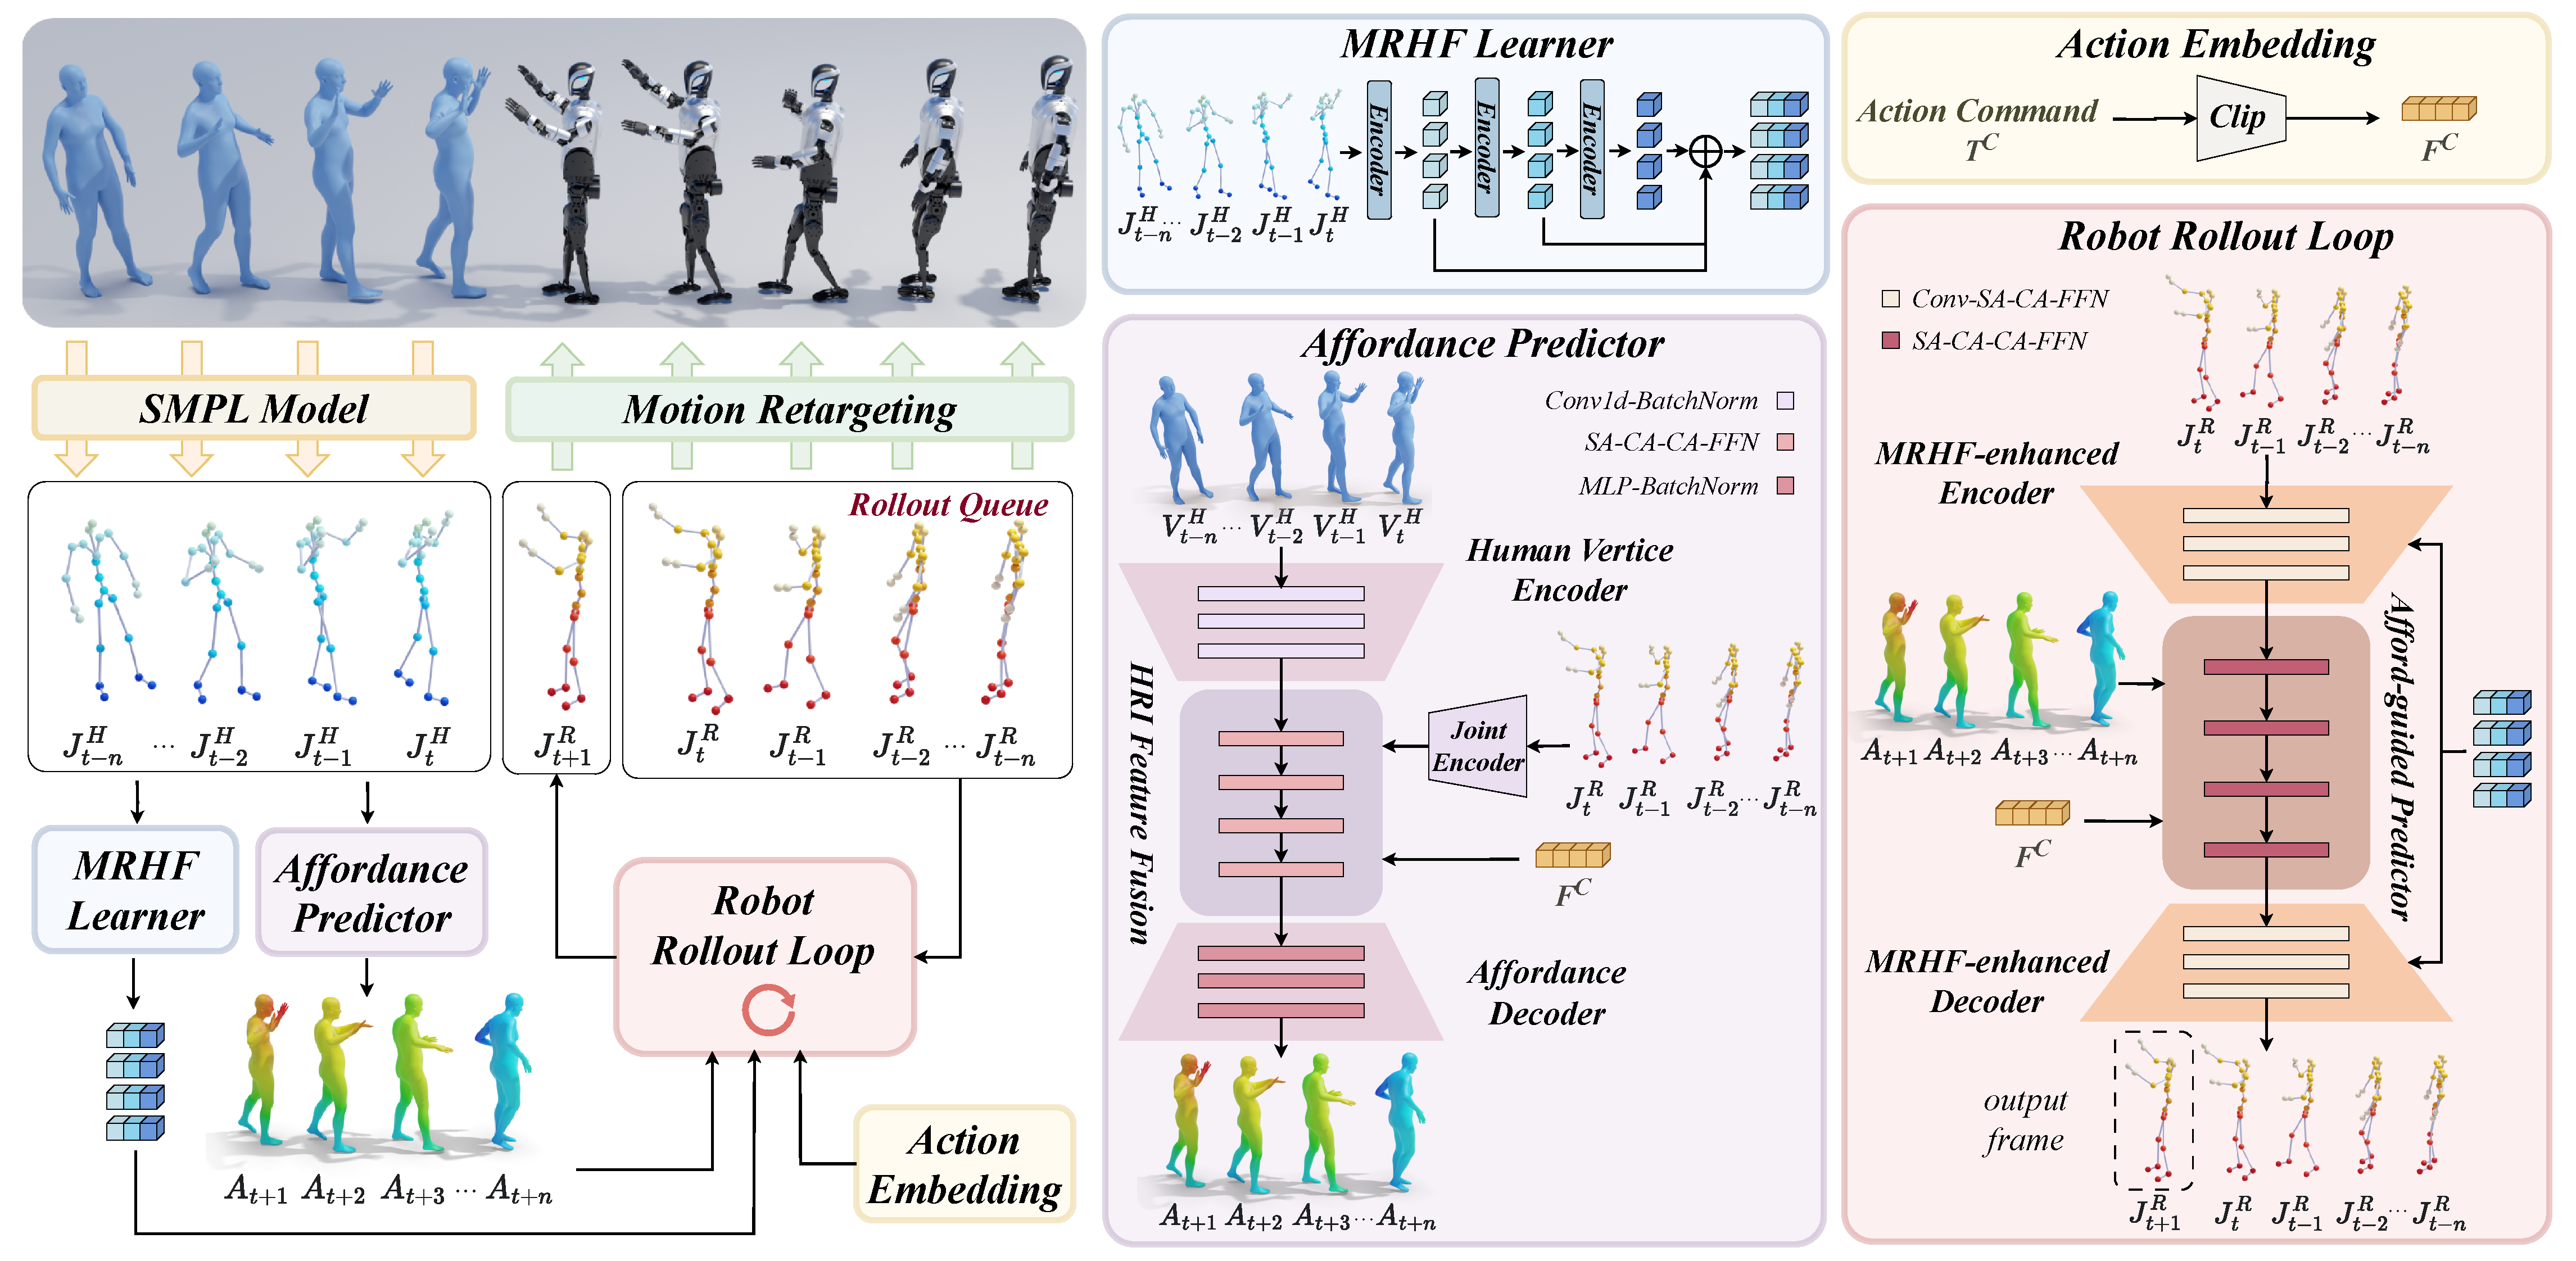
\includegraphics[width=1\linewidth]{images/intermodel-mainv5.pdf}
\vspace{-20pt}
\caption{Overall pipeline of our Robotic Interaction Model. The model ingests text action commands, historical robot joints, observed human joints and SMPL mesh vertices, and processes them through four tightly coupled modules. The Affordance Predictor explicitly estimates dense end-effector–vertex spatial fields to enable dexterous, socially-appropriate contact reasoning; the Multi-Resolution Human Feature (MRHF) Learner fuses hierarchical temporal cues to boost situational awareness; the Robot Rollout Loop leverages these affordance and human features to iteratively generate coherent, context-adaptive joint trajectories for real-time responsiveness; and finally, the Motion Retargeting module maps each predicted skeleton frame to robot-specific angle axis.}
\label{fig:interactiveModel}
\vspace{-10pt}
\end{figure*}
% Real-time, context-aware motion generation remains a challenging problem in human-robot interaction, especially in dynamic and contact-rich scenarios. Prior works~\cite{wang2021multi,xu2024regennet,mueller2024massively} often lack sufficient responsiveness and realistic interaction dynamics.

% To address these challenges, we propose a novel Robotic Interaction Model capable of generating coherent and timely humanoid robot motions for seamless human-robot interactions. Our model is composed of three main modules:

% \begin{itemize}
%     \item \textbf{Affordance Predictor}, which captures fine-grained spatial relationships between robot end-effectors and human body vertices, guiding precise and socially appropriate interactive actions.
%     \item \textbf{Multi-Resolution Human Feature (MRHF) Learner}, which extracts hierarchical temporal features from human motion to enhance situational awareness and response diversity.
%     \item \textbf{Robot Rollout Loop}, which generates robot motions in a frame-by-frame manner to ensure real-time responsiveness and long-term stability.
% \end{itemize}

% \subsection{Model Input and Output}

% Our model generates robot motions online by conditioning on three inputs at each timestep (Fig.~\ref{fig:interactiveModel}): 

% (1) a textual command \(T^C\), representing the intended interaction (e.g., \textit{``High-five''}, \textit{``Handshake''}); 

% (2) historical robot joint skeletons \(J^{R}_{t-n \sim t}\), encoding recent robot motion; 

% (3) observed human motion, including joint skeletons \(J^{H}_{t-n \sim t}\) and SMPL mesh vertices \(V^{H}_{t-n \sim t}\), derived from pose and translation parameters from motion capture (Section ~\ref{sec:mocap}).

% These inputs provide both semantic intent and physical interaction context, enabling the model to predict a short sequence of future robot joint skeletons \(J^{R}_{t+1 \sim t+k}\), because sequence supervision can benefit the consistency of predicted robot motion. However, only the immediate next frame \(J^{R}_{t+1}\) is executed and appended to the rollout queue for the next prediction. This frame-by-frame rollout strategy is crucial for:

% \begin{itemize}
%     \item \textbf{Responsiveness}: adapting to rapid or unexpected changes in human behavior;
%     \item \textbf{Robustness}: mitigating error accumulation common in offline motion generation;
%     \item \textbf{Coherence}: maintaining consistent and fluid robot behavior by conditioning on updated observations each step.
% \end{itemize}

% This mechanism mirrors human interactive behavior, continuously adjusting actions based on perceptual feedback.

% \subsection{Semantic Action Embedding}

% To embed semantic intent, the input command \(T^C\) is encoded into a compact action feature \(F^C\) using a pre-trained CLIP text encoder~\cite{radford2021learning}. This embedding guides downstream modules in generating context-aware motions aligned with the intended interaction.

% \subsection{Affordance Predictor Module}

% Physical and social interactions require precise knowledge of where and how a robot should contact a human. Our Affordance Predictor models a dense spatial affordance field that estimates distances between robot end-effectors (robot hands) and every human body vertex, enabling fine-grained contact reasoning.

% The module encodes the human SMPL mesh sequence \(V^H_{t-n \sim t}\) with a PointNet-based Human Vertice Encoder, generating vertex-wise features \(F^{V^H}_{t-n \sim t}\). These features are fused with the robot’s motion history \(J^R_{t-n \sim t}\) and action embedding \(F^C\) via an encoder-decoder transformer to produce refined interaction features. An MLP-based Affordance Decoder then outputs the dense affordance field \(A_{t+1 \sim t+k}\), informing the robot where to interact in a socially appropriate and physically feasible manner.

% \subsection{MRHF Learner Module}

% Human behavior is temporally hierarchical, with cues evolving at different speeds. To capture this, the MRHF Learner extracts multi-resolution features from the human skeleton sequence \(J^{H}_{t-n \sim t}\) using stacked convolutional and transformer layers. These features encode short-term nuances and long-term behavioral intent, which are concatenated to form the Multi-Resolution Human Feature \(F^{H_{MR}}_{t-n \sim t}\).

% The MRHF enhances the robot's ability to synthesize responses that are temporally coherent and contextually relevant, allowing adaptation to sudden changes while maintaining smooth interaction flow.

% \subsection{Robot Rollout Loop Module}

% To generate natural and responsive robot motions, the Robot Rollout Loop synthesizes actions frame-by-frame, avoiding the error accumulation of offline full-sequence prediction.

% Within this loop, an MRHF-enhanced Encoder processes historical robot motion \(J^{R}_{t-n \sim t}\) together with human features \(F^{H_{MR}}_{t-n \sim t}\) to extract context-aware representations \(F^{R}_{t-n \sim t}\). These are combined with affordance predictions \(A_{t+1 \sim t+k}\) and action embedding \(F^C\) via an Affordance-guided Predictor, yielding spatially aware features \(F^{R'}_{t+1 \sim t+k}\).

% A corresponding MRHF-enhanced Decoder then generates future robot joint sequences \(J^{R}_{t+1 \sim t+k}\). Only the immediate next pose \(J^{R}_{t+1}\) is forwarded to the Motion Retargeting Module for execution and rollout updates.

% This iterative process ensures the robot's motions remain coherent over time while adapting fluidly to evolving human actions.

% \subsection{Robot Motion Retargeting}

% The final predicted joint skeletons are transformed into robot-specific motion parameters using a retargeting module. This module employs a transformer-based spatial encoder capturing inter-joint relationships, followed by a bidirectional GRU that models temporal dynamics. The result is smooth, physically plausible robot motion suitable for execution on the target platform.


% Overall, our Robotic Interaction Model effectively balances real-time responsiveness, motion coherence, and social appropriateness, enabling natural and seamless human-robot interactions in dynamic environments.








%\input{sections/4-2-HR-collaboration}
\section{System Evaluation}
\begin{table*}[]
\centering

\resizebox{\linewidth}{!}{ 
\tiny\begin{tabular}{c|c|cccccccccc}
\hline
Setting                     & Finetune Scale                                               & PA-MPJPE↓ & MPJPE↓ & Traj↓ & Orie↓ & C\_prec↑ & C\_rec↑ & C_acc↑& C_F1↑ & FID↓ & R-score↑ \\ \hline
\multirow{4}{*}{Cross Domains} & Base        &   4.57        &       17.12    &    0.286     &   28.14  &  0.891   &     0.773      &    0.807     &     0.828    &     0.289     &     /      \\ \cline{2-12} & $\sim$100         &    \textcolor[rgb]{0.07,0.55,0.15}{4.44}       &    \textcolor[rgb]{0.07,0.55,0.15}{16.32}       &    \textcolor[rgb]{0.07,0.55,0.15}{0.280}      &   \textcolor[rgb]{0.07,0.55,0.15}{26.86}  &  \textcolor[rgb]{0.07,0.55,0.15}{ 0.908}  &     \textcolor[rgb]{0.07,0.55,0.15}{0.774}      &         \textcolor[rgb]{0.07,0.55,0.15}{0.817}   &    \textcolor[rgb]{0.07,0.55,0.15}{ 0.836 }     & \textcolor[rgb]{0.07,0.55,0.15}{0.241}   &   /   \\ \cline{2-12}& $\sim$1000         &   \textcolor[rgb]{0.07,0.55,0.15}{4.30}     &     \textcolor[rgb]{0.07,0.55,0.15}{15.67}      &     \textcolor[rgb]{0.07,0.55,0.15}{0.275}      &      \textcolor[rgb]{0.07,0.55,0.15}{25.38}     &    \textcolor[rgb]{0.07,0.55,0.15}{0.918}    &    \textcolor[rgb]{0.77,0.15,0.32}{0.754}     &      \textcolor[rgb]{0.07,0.55,0.15}{0.812}     &      \textcolor[rgb]{0.07,0.55,0.15}{0.828}     &    \textcolor[rgb]{0.07,0.55,0.15}{0.202}      &      /    \\ \cline{2-12}& $\sim$10000   &      \textcolor[rgb]{0.07,0.55,0.15}{\textbf{3.85}}    &      \textcolor[rgb]{0.07,0.55,0.15}{\textbf{14.04}}     &    \textcolor[rgb]{0.07,0.55,0.15}{\textbf{0.232}}    &    \textcolor[rgb]{0.07,0.55,0.15}{\textbf{21.78}}     &    \textcolor[rgb]{0.07,0.55,0.15}{\textbf{0.923}}   &    \textcolor[rgb]{0.07,0.55,0.15}{\textbf{0.805}}  &     \textcolor[rgb]{0.07,0.55,0.15}{\textbf{0.842}}     &   \textcolor[rgb]{0.07,0.55,0.15}{\textbf{0.860}}   &    \textcolor[rgb]{0.07,0.55,0.15}{\textbf{0.094}}    &     /     \\ \hline
\multirow{4}{*}{Cross Categories} & Base &   3.06        &       10.72    &     0.151     &   34.49  &  0.822   &     0.845      &    0.807     &     0.833    &     0.274      &     0.448  \\ \cline{2-12}& $\sim$100         &     \textcolor[rgb]{0.07,0.55,0.15}{3.00}      &      \textcolor[rgb]{0.07,0.55,0.15}{10.52}     &     \textcolor[rgb]{0.07,0.55,0.15}{0.150}     &   \textcolor[rgb]{0.07,0.55,0.15}{34.20}  &  \textcolor[rgb]{0.77,0.15,0.32}{0.817}   &      \textcolor[rgb]{0.07,0.55,0.15}{0.849}     &  \textcolor[rgb]{0.77,0.15,0.32}{ 0.806 }     &     \textcolor[rgb]{0.77,0.15,0.32}{0.833}    &    \textcolor[rgb]{0.07,0.55,0.15}{ 0.262}      &    \textcolor[rgb]{0.07,0.55,0.15}{0.451 }      \\ \cline{2-12}& $\sim$1000         &    \textcolor[rgb]{0.07,0.55,0.15}{2.88}    &       \textcolor[rgb]{0.07,0.55,0.15}{10.06}    &     \textcolor[rgb]{0.07,0.55,0.15}{ 0.143}     &    \textcolor[rgb]{0.07,0.55,0.15}{32.08}       &   \textcolor[rgb]{0.07,0.55,0.15}{ 0.826}    &    \textcolor[rgb]{0.07,0.55,0.15}{\textbf{0.850}}   &       \textcolor[rgb]{0.07,0.55,0.15}{0.813 }   &     \textcolor[rgb]{0.07,0.55,0.15}{0.838}      &    \textcolor[rgb]{0.07,0.55,0.15}{0.241 }      &    \textcolor[rgb]{0.07,0.55,0.15}{0.455}      \\ \cline{2-12}& $\sim$10000   &  \textcolor[rgb]{0.07,0.55,0.15}{\textbf{2.67}}     &    \textcolor[rgb]{0.07,0.55,0.15}{\textbf{9.34}}       &    \textcolor[rgb]{0.07,0.55,0.15}{\textbf{13.05}}     &    \textcolor[rgb]{0.07,0.55,0.15}{ \textbf{30.02}}      &     \textcolor[rgb]{0.07,0.55,0.15}{\textbf{0.841}}   &     \textcolor[rgb]{0.07,0.55,0.15}{0.847}   &      \textcolor[rgb]{0.07,0.55,0.15}{\textbf{0.822}}    &    \textcolor[rgb]{0.07,0.55,0.15}{\textbf{0.844}}   &    \textcolor[rgb]{0.07,0.55,0.15}{\textbf{0.208}}    &      \textcolor[rgb]{0.07,0.55,0.15}{\textbf{0.465}}    \\ \hline
\end{tabular}
}
\caption{Results of interaction skill enhancement across different settings with varying finetune scales. \textcolor[rgb]{0.77,0.15,0.32}{Red} indicates a decrease while \textcolor[rgb]{0.07,0.55,0.15}{Green} indicates an increase relative to Base. Due to extreme category imbalance in Inter-Human, R-score is not applicable in \textit{Cross-Domain} setting.}
\vspace{-4ex}
\label{tab:finetune}
\end{table*}
We conduct system evaluation by assessing whether it meets the design goals. Accordingly, our experiments focus on answering three questions, presented in Sections~\ref{eval1}, \ref{eval2}, \ref{eval3}, respectively.

A. Does the interactive model produce reasonable and plausible robot reactions that ensure natural and smooth interactions?

B. Does the system support real-time and realistic interaction experience that helps humans adapt to human-robot interactions?

C. Does the system facilitate data collection and efficient fine-tuning that continuously enhance robot interaction skills?

\subsection{Evaluation of Interactive Model}
\label{eval1}
\noindent\textbf{Datasets.}
The Ground Truth (GT) data for training and evaluating our model was generated from the large-scale human-human interaction dataset, Inter-X \cite{xu2024inter}, addressing the lack of a comparable human-robot dataset. The GT generation process involved treating one human's motion in an interaction pair as the input, while the second human's response was converted into the target robot motion using an \textbf{offline motion retargeting} pipeline. This pipeline employs the kinematics-based methodology from Human2Humanoid \cite{he2024learning} to map human movements to the specific constraints of our robot models (LEJU Kuavo \cite{lejukuavorobot} and Unitree H1 \cite{unitreeh1robot}) ensuring the resulting motion is physically plausible and serves as a high-quality supervision signal. This offline generation of GT is distinct from the online, learning-based \textbf{Robot Motion Retargeting Module (Sec. 5.5)}, which is trained using this data to perform real-time predictions. Through this procedure, we created the \textit{Inter-HRI} benchmark for our experiments, which retains the original train-test split from Inter-X and is downsampled to 10FPS to suit our motion capture setup. For a comprehensive walkthrough of the GT dataset generation, please refer to the \textbf{Supplementary Material, Section 3.1}.
% No existing dataset specifically targets human-robot interaction. Therefore, we adapt human-human interaction data to HRI %by
% for enabling robots to learn realistic behaviors. We introduce \textit{Inter-HRI} by extending the Inter-X dataset~\cite{xu2024inter}, which focuses on human-human interaction.
% \textbf{Inter-HRI} is created by mapping one subject’s angle-axis parameters to specific robot joint representation like Unitree H1~\cite{unitreeh1robot} and LEJU Kuavo~\cite{lejukuavorobot}, following% PHC
% ~\cite{luo2023perpetual}. It retains the original train-test split and is downsampled to 10FPS to suit our motion capture setup.


\noindent\textbf{Evaluation Metrics.} 
For measuring action precision, MPJPE is the mean per joint position error and PA-MPJPE aligns predictions via Procrustes analysis (rotation, translation, scale) before computing error~\cite{deitke2020robothor}. Both are reported in centimeters. Traj measures root joint trajectory error (\textit{cm}), while Orie measures orientation error(\textit{deg}).
For measuring contact quality, we use dimensionless metrics: precision ($C_{\text{prec}}$), recall ($C_{\text{rec}}$), accuracy ($C_{\text{acc}}$), and F1 score ($C_{\text{F1}}$).
For measuring generative fidelity, FID calculates Fréchet distance between inception network features. R-score evaluates text-motion alignment via Euclidean distances between embeddings and Top-3 retrieval accuracy. 
%Both are dimensionless.

%~\cite{dai2024motionlcmrealtimecontrollablemotion}
%~\cite{li2023object}
% \textbf{Min dist.}, \textbf{Pelvis dist.}, and \textbf{All dist.}~\cite{wang2024move} compute normalized distances from human mesh vertices to robot hand joints, quantifying affordance map accuracy in \textit{centimeters}. Lower distances indicate better performance.

\noindent\textbf{Comparison.}
\label{sec:baseline}
We compare our Robotic Interaction Model against four recent state-of-the-art methods, all re-implemented or fine-tuned and evaluated fairly on the Inter-HRI benchmark.
As shown in Fig.~\ref{fig:visintermodel-comp} and Tab.~\ref{tab:hhi}, our model consistently outperforms these baselines with the lowest PA-MPJPE and MPJPE, and significant improvements in contact metrics ($C_{\text{prec}}$, $C_{\text{F1}}$), FID, and R-score, indicating superior spatial accuracy, physical realism, and semantic consistency.
These improvements result from our %Multi-Resolution Human Feature (
MRHF Learner, which captures hierarchical temporal behavior, and the Affordance Predictor, enabling precise, socially-aware contact reasoning (details in supplementary material). Together, they enable realistic, contextually adaptive, and real-time human-robot interactions. More our results of diverse interaction types are presented in Fig.~\ref{fig:visintermodel-ours}.
%Overall, the results emphasize the importance of multi-scale behavior modeling and dense affordance mapping for seamless human-robot collaboration.

\noindent\textbf{Human Evaluation.}We also compared the quality of generated actions across ten representative action types in the Inter-X dataset using a 5-point Likert scale, where a higher score indicates a more natural and accurate result. 30 computer science students (15 male, 15 female) were asked to rate the outputs of five methods: JRT, MRT, ReGenNet, SAST, and our proposed approach. The results show that our method significantly outperforms the baselines, achieving an average score of 4.5, while the closest competitor, JRT, received an average of 2.46. MRT and ReGenNet followed with average scores of 2.1 and 1.86, respectively, and SAST ranked lowest with 1.64. These findings suggest that our approach generates actions that are perceived by humans as more realistic and semantically appropriate than those produced by existing methods.



% We compare our method with four representative baselines that cover a wide spectrum of recent advances in multi-person motion prediction and interactive human-robot motion synthesis:
% JRT~\cite{xu2023joint}: Models explicit joint relations for multi-person motion prediction.
% MRT~\cite{wang2021multi}: Combines local and global dynamics via dual Transformers.
% ReGenNet~\cite{xu2024regennet}: Diffusion-based action-reaction synthesis for interactive scenarios.
% SAST~\cite{mueller2024massively}: Integrates scene and social context for long-term, multi-person motion forecasting.
% All baselines are re-implemented or tuned following the official protocols on the Inter-HRI benchmark for fair comparison.

% Experimental results (see Tab. 1) show that our approach achieves a new state-of-the-art across all evaluation metrics on the Inter-HRI benchmark, consistently outperforming these strong baselines. Notably, our model achieves the lowest PA-MPJPE and MPJPE scores, reflecting superior spatial accuracy in joint prediction. In addition, our method demonstrates remarkable improvements in contact-related metrics (C_prec, F1), perceptual realism (FID), and semantic consistency (R-score).

% We attribute these advances to our model's core innovations: the Multi-Resolution Human Feature (MRHF) Learner, which captures hierarchical temporal cues from human behavior, and the Affordance Predictor, which enables fine-grained, socially-appropriate contact reasoning. The synergy between these modules allows our system to bridge the gap between physical realism, social appropriateness, and online adaptability—enabling highly realistic and contextually adaptive human-robot interactions.

% In summary, the results underscore the importance of modeling both multi-scale human behavior and dense affordance maps for achieving seamless, real-time human-robot collaboration.



% \subsubsection{Ablation Study}

% $$\\$$
% Modifying

% Tab.~\ref{tab:ab-hoi} demonstrates the necessity of both the MRHF Learner and the Affordance Predictor. Removing either module leads to a clear degradation in core metrics. MRHF brings substantial gains in motion accuracy (PA-MPJPE/MPJPE), validating our motivation to capture multi-scale human dynamics. The Affordance Predictor Module further improves orientation, trajectory, and motion realism (Orie, Traj, FID), confirming its role in producing interaction-aware and semantically meaningful robot behavior. Combining both, our full model achieves the best performance across all aspects—including spatial precision and motion coherence—highlighting the complementary strengths and the effectiveness of our design.



\subsection{Evaluation of Real-Time and Realistic HRI}
\label{eval2}

\noindent\textbf{Time Performance.} Our system involves a 10FPS LiDAR device, a host server running the motion capture and interactive model, and display ends, either an AR glass or a notebook for different perspectives.
%The LiDAR device works at a 10FPS frequency. The host server runs the motion capture and interactive model, then broadcasts robot motions to
%the display ends, either an AR glass or a notebook for different perspectives. 
%, instantly receives the pose sequence and drives the robot character for visualization. 
All modules run in parallel with cached queues between them.
On a host server with an i9-14900kf CPU and a Nvidia A6000 GPU, it achieves a speed of 40FPS with overall latency less than 0.2sec.

\noindent\textbf{Quality Performance.} %Our system captures human motions as the input of the robotic interaction model and present its generated robot motions to human users. 
%We then examine the quality performance of our platform in terms of human-robot interaction. That is, given the interactive model with the above quantitative evaluation, how does our platform effectively leverage this model's capabilities? 
In our system, the Ouster-1-128 LiDAR exhibits a scanning error of $\pm$1-3$\,cm$ in indoor environments. For motion capture, we employ a noise-resistant algorithm, which achieves a human keypoint estimation error of $6.2~cm$ and a joint angle error of $15.40~degree$ (evaluated on the FreeMotion %indoor 
dataset). These errors define the input data error for the interaction model. On the other hand, %since the predicted robot reactions are converted as pose sequences to the display ends, we compute 
between the robot predicted by the interactive model and that presented to the user, i.e. input and output of the retargeting module, the joint angle error is $3.80~degree$ for LEJU Kuavo and $6.81~degree$ for Unitree H1 in the Inter-HRI dataset.
% \color{blue}Given the scanning error of the LiDAR(Ouster-1-128) device within $+-1-2cm$ in indoor scenes and the motion capture algorithm produces pose parameter error within xxx, we assess that the error of the captured human behavior, i.e. input of interactive model, is about xxx. \color{black} \color{purple}On the other hand, since the predicted robot reactions are converted as pose sequences to the display ends, we compute the error between the robot predicted by the interactive model and that presented to the user. Their average keypoint distance is within xxx, indicating that the predicted robot reactions are reliably conveyed to human users to enable the realistic and real-time human-robot interaction. %Thus the collected user ratings during the human-robot interaction process would provide authentic feedback for the interactive model.
\color{black}

\noindent\textbf{User Empirical Test.} To evaluate our system, we recruited a total of 50 participants (33 male, 17 female), aged between 18 and 56 years and ranging in height from 162 cm to 191 cm, with diverse academic and professional backgrounds in robotics, computer graphics, and augmented reality. Each participant required to test 5 types of interaction 3 iterations per type. %For each human-robot interaction, the user is informed of the interaction type and an appropriate initial position to ensure that LiDAR can perceive human motion during the following interaction process. Then the user wear the AR glasses and click the "connect" button to start. 
After the interactions, the user rates their interaction experience on a 5-Likert scale from different dimensions, where 1 indicates "poor" and 5 indicates "excellent".
Among the dimensions, 
%We collect user ratings of the platform's performance from the following aspects. 
\emph{interaction completion} reflects how well the user considers the interaction as successfully completed. \emph{Realism} is whether the user perceives a realistic visualization and a vivid interaction with the virtual robot. \emph{Rationality} and 
\emph{fidelity} measure whether the robot's reaction can interact with the human user appropriately and whether it acts like a physical humanoid robot. \emph{Real-time performance} is whether the user considers the robot's reaction as smooth and timely. 
\emph{Usability} and \emph{willing-to-use} reflects whether the users view the system as easy-to-use and would like to continue performing the human-robot interaction via our system.

The process and statistics are presented in Fig.~\ref{fig:systeminter} and~\ref{fig:userstudy}. All dimensions receive average ratings above the moderate level. Our system exhibits high realism and moderate real-time characteristics, as well as positive rationality and fidelity, yet distinguishable from real human-human interactions. More importantly, most users consider our system as quite easy-to-use and would like to continue using it. 

\noindent\textbf{Real Robot Test.} %We further examine the physical fidelity of the robot's reactions during the human-robot interaction. First, to conduct the physical simulation test, we adapt a perceptual humanoid controller [] to our robot model, \color{red}including xx and xx\color{black}, and train the policy network using reinforcement learning in Isaac gym. The policy network can drive the robot model to align with a specified action sequence as much as possible while strictly ensuring the physical feasibility constraints. \color{gray}We use the trained controller to perform the robot's reactions produced by the interactive model during the user empirical testing in the simulation environment. It turns out that the simulated robot movements exhibit an error within xxx compared to the predicted robot reactions, indicating the high physical fidelity of the movements of the virtual robot.\color{black}
We deploy the virtual robot reactions to a real LEJU Kuavo robot. That is, we preserve the exact upper body movements and body center trajectory, and slightly tune the lower body movements with its default offline simulator software to maintain the robot's balance. As in Fig. ~\ref{fig:realrobot}, the appearance and movement of the real robot exhibits a high consistency with that presented by our system. This test indicates that the human-robot interaction experience via our system is reliable enough to assist human users in getting used to interacting with robots in the real world.

\noindent\textbf{Discussion.} Our system currently supports a single active user, although the motion capture module can track multiple individuals. For reliable operation, users must remain within the LiDAR’s line of sight and unobstructed by obstacles. If no human is detected, the prediction pipeline pauses and the robot remains visible but stationary in the AR interface, thereby preventing unintended behaviors while maintaining scene continuity.


\subsection{Evaluation of Robot Interaction Skill Enhancement}
\label{eval3}

\noindent\textbf{Setup.} We conduct model adaptation with a base model trained on a subset of Inter-HRI with 20 basic actions. The fine-tuning uses the loss function leveraging both positive and negative samples 
\[
L = L_{\text{pos}} - \alpha L_{\text{neg}},
\]
where $L_{\text{pos}}$  and $L_{\text{neg}}$ are reconstruction loss terms to encourage learning from desirable interactions while penalizing undesired behaviors, and $\alpha$ controls the negative loss influence.


We evaluate two settings by processing existing datasets to mimic the interactions collected with our system. \textit{Cross Categories} focuses on interactions outside the 20 base types. \textit{Cross Domain} simulate real-world user movements by filtering samples of these types from another interaction dataset InterHuman~\cite{liang2024intergen}. 
%
In both settings, we use 1:1 positive and negative samples. Negative samples are produced by (1) injecting random noise to robot motions, (2) making static sequences like robot not responding to humans, and (3) re-pairing human-robot movements like mismatched interactions.

\noindent\textbf{Results.}
Tab.~\ref{tab:finetune} presents the quantitative results for \emph{Cross Categories} and \emph{Cross Domain}.
Increasing data scale (to 100, 1,000, 10,000 samples) consistently improves performance on both settings. These improvements confirm that our model adaptation mechanism can effectively utilize
various human-robot interaction data collected with our system to enhance robot interaction skills.

%To enable the continuous enhancement of the robot’s interaction skills and facilitate its adaptive behaviors to user preferences, we employ a feedback-driven model adaptation mechanism.

%\noindent\textbf{Setup.}
%The model adaptation is based on the model trained on a subset of \textit{Inter-HRI}, which includes 20 base actions. Our basic loss function is elaborated in the supplementary. The adaptation process uses a modified one, incorporating positive and negative samples:
%$
%L = L_{\text{pos}} - \alpha L_{\text{neg}},
%$
%where $L_{\text{pos}}$ and $L_{\text{neg}}$ are positive and negative losses, respectively, and $\alpha$ controls the negative loss influence. It encourages learning from desirable interactive behaviors while penalizing undesired ones.

%\noindent\textbf{Setting Construction.}
%We constructed two model adaptation settings. \textit{Cross Categories} focuses on actions outside the basic 20 actions. \textit{Cross Domains} evaluates generalization to unseen patterns by filtering samples from another interaction dataset InterHuman~\cite{liang2024intergen} related to basic actions. 
%In all settings, positive and negative samples are balanced 1:1. Positive samples come from GT. Negative samples are randomly sampled from (1) noise sequences with no valid interaction, (2) static sequences with no robot response, and (3) mismatched human-robot pairs.

%\noindent\textbf{Results.}
%Table.~\ref{tab:finetune} presents the quantitative results for Cross-Domain and Cross-Category settings, where increasing model adaptation data scale (100, 1,000, 10,000 samples) consistently improves the performance. 
%%For example, in Cross Categories, PA-MPJPE decreases from 3.06 to 2.67 and FID from 0.274 to 0.208, indicating enhanced spatial accuracy and perceptual fidelity. %
%These improvements confirm that our model adaptation design enables more robust and adaptable robot interaction skills.


% \subsection{Evaluation of Robot Interaction Skill Enhancement}
% \label{eval3}

% \subsubsection{Finetuning Setup}
% To enable the continuous enhancement of the robot's interaction skills and facilitate its adaptive behaviors to user preferences, we employ a finetuning mechanism. This mechanism is a core component of our model adaptation cycle, leveraging human feedback collected during human-robot interactions.

% \paragraph{Loss Function}
% Our finetuning process utilizes a modified loss function that explicitly incorporates both positive and negative samples. The loss function is defined as:
% $$L = L_{pos} - A L_{neg}$$
% where $L_{pos}$ represents the positive loss, $L_{neg}$ represents the negative loss, and $A$ is a coefficient used to constrain the influence of the negative loss. This formulation encourages the model to learn from desirable interactions ($L_{pos}$) while actively penalizing undesirable or incorrect behaviors ($L_{neg}$).

% \paragraph{Dataset Construction for Finetuning}
% We constructed two distinct types of datasets to comprehensively evaluate and improve the finetuned model's performance: `Cross Categories` and `Out Domain`.

% \textbf{Finetune - Cross Categories:} This dataset focuses on actions *outside* the initial 20 actions selected for the base training set of our interaction model.
% \begin{itemize}
%     \item \textbf{Sample Selection:} Positive and negative samples are selected in a 1:1 ratio, consistent with the official InterX training set division.
%     \item \textbf{Negative Sample Types:} To diversify the negative samples and robustly train the model to avoid erroneous interactions, we incorporated three distinct types of negative samples:
%     \begin{enumerate}
%         \item \textbf{Noise Samples:} Randomly generated or perturbed interaction sequences that do not correspond to any valid human-robot interaction.
%         \item \textbf{Static Samples:} Sequences where the robot remains motionless or exhibits no reactive behavior despite human input, representing a lack of interaction.
%         \item \textbf{Incorrectly Paired Interaction Samples:} Sequences where a valid human action is randomly paired with an inappropriate or mismatched robot response from the dataset.
%     \end{enumerate}
%     \item \textbf{Dataset Scaling:} From approximately 30,000 segmented samples derived from original sequences, we created finetuning sets of varying scales to evaluate the impact of data quantity: 100ft, 1000ft, and 10000ft. These sets were generated by shuffling the 30,000 samples and taking the first 100, 1000, and 10000 samples, respectively.
%     \item \textbf{Test and Validation Sets:} Corresponding test and validation sets were constructed for actions outside the 20 base actions, adhering to the official InterX test and validation set divisions.
% \end{itemize}

% \textbf{Finetune - Out Domain:} This dataset evaluates the model's generalization capabilities to unseen interaction patterns, simulating real-world data collection from users.
% \begin{itemize}
%     \item \textbf{Dataset Source:} We utilized the InterHuman training set as the source.
%     \item \textbf{Sample Filtering:} Samples were filtered to include only those corresponding to the 40 InterX actions, with a specific focus on the parts belonging to the initial 20 actions of our base training set. This simulates the collection of user feedback data within the context of the SymbioSim platform.
%     \item \textbf{Test and Validation Sets:} The InterHuman test and validation sets were similarly filtered and used for evaluation in this out-domain scenario.
% \end{itemize}

% Our experimental findings consistently demonstrate that finetuning with both positive and negative samples significantly enhances the model's performance. Furthermore, the efficacy of this finetuning process is positively correlated with the quantity of training samples, indicating that more extensive user feedback leads to a more robust and adaptable robot interaction model.


% \subsubsection{Results}
% \label{sec:results}
% We evaluate its efficacy across varying scales of finetuning data (100, 1000, 10000 samples). Tab.~\ref{tab:finetune} presents the quantitative results for "Cross Categories" and "Cross Domain" settings.

% \textbf{Cross Categories:} This setting focuses on actions outside the base model's initial training set. As finetune scale increases, we observe consistent performance enhancements:
% \begin{itemize}
%     \item Error metrics (PA-MPJPE, MPJPE, Traj, Orie, FID) show significant reduction. For instance, PA-MPJPE improves from 3.06 (Base) to \textbf{2.67} with 10000 finetune samples, and MPJPE from 10.72 to \textbf{9.34}. FID decreases from 0.274 to \textbf{0.208}.
%     \item Accuracy-based metrics (C\_prec, C\_rec, C\_acc, C\_F1, R-score) generally increase, indicating improved contact and interaction quality. C\_acc rises from 0.807 to \textbf{0.822}, and C\_F1 from 0.833 to \textbf{0.844}. R-score, reflecting overall interaction quality, improves from 0.448 to \textbf{0.465}.
% \end{itemize}

% \textbf{Cross Domain:} This evaluates generalization to unseen interaction patterns, simulating real-world user data. While R-score is not applicable due to extreme category imbalance, other metrics demonstrate similar trends:
% \begin{itemize}
%     \item Error metrics exhibit substantial improvements. PA-MPJPE drops from 4.57 (Base) to \textbf{3.85} with 10000 finetune samples, and MPJPE from 17.12 to \textbf{14.04}. Notably, FID shows a drastic reduction from 0.289 to \textbf{0.094}, indicating superior fidelity in generated motions within novel domains.
%     \item Contact accuracy metrics generally improve, with C\_prec rising from 0.891 to \textbf{0.923}, C\_rec from 0.773 to \textbf{0.805}, C\_acc from 0.807 to \textbf{0.842}, and C\_F1 from 0.828 to \textbf{0.860}.
% \end{itemize}

% Overall, these results consistently demonstrate that finetuning with positive and negative samples significantly enhances the robot's interaction skills and adaptability. The performance gains are directly correlated with the quantity of finetuning data, validating SymBridge's model adaptation cycle as an effective mechanism for continuous improvement through human feedback.



% \begin{table*}[t]
% \caption{Results of interaction skill enhancement across different settings with varying finetune scales. Red indicates a decrease while Green indicates an increase relative to Base. Due to extreme category imbalance, R-score is not applicable in Cross Domain setting.}
% \label{tab:results}
% \centering
% \resizebox{\linewidth}{!}{%
% \begin{tabular}{|l|l|c|c|c|c|c|c|c|c|c|c|}
% \hline
% \textbf{Setting} & \textbf{Finetune Scale} & \textbf{PA-MPJPE$\downarrow$} & \textbf{MPJPE$\downarrow$} & \textbf{Traj$\downarrow$} & \textbf{Orie$\downarrow$} & \textbf{C\_prec$\uparrow$} & \textbf{C\_rec$\uparrow$} & \textbf{C\_acc$\uparrow$} & \textbf{C\_F1$\uparrow$} & \textbf{FID$\downarrow$} & \textbf{R-score$\uparrow$} \\
% \hline
% Base & & 4.57 & 17.12 & 0.286 & 28.14 & 0.891 & 0.773 & 0.807 & 0.828 & 0.289 & \\
% \multirow{3}{*}{Cross Domain} & \textasciitilde{}100 & 4.44 & 16.32 & 0.280 & 26.86 & 0.908 & 0.774 & 0.817 & 0.836 & 0.241 & \\
% & \textasciitilde{}1000 & 4.30 & 15.67 & 0.275 & 25.38 & 0.918 & 0.754 & 0.812 & 0.828 & 0.202 & / \\
% & \textasciitilde{}10000 & \textbf{3.85} & \textbf{14.04} & \textbf{0.232} & \textbf{21.78} & \textbf{0.923} & \textbf{0.805} & \textbf{0.842} & \textbf{0.860} & \textbf{0.094} & / \\
% \hline
% Base & & 3.06 & 10.72 & 0.151 & 34.49 & 0.822 & 0.845 & 0.807 & 0.833 & 0.274 & 0.448 \\
% \multirow{3}{*}{Cross Categories} & \textasciitilde{}100 & 3.00 & 10.52 & 0.150 & 34.20 & 0.817 & 0.849 & 0.806 & 0.833 & 0.262 & 0.451 \\
% & \textasciitilde{}1000 & 2.88 & 10.06 & 0.143 & 32.08 & 0.826 & 0.850 & 0.813 & 0.838 & 0.241 & 0.455 \\
% & \textasciitilde{}10000 & \textbf{2.67} & \textbf{9.34} & \textbf{0.135} & \textbf{30.02} & \textbf{0.841} & \textbf{0.847} & \textbf{0.822} & \textbf{0.844} & \textbf{0.208} & \textbf{0.465} \\
% \hline
% \end{tabular}%
% }
% \end{table*}





% \begin{table*}[]
% \centering

% \resizebox{\linewidth}{!}{ 
% \begin{tabular}{c|c|cccccccccc}
% \hline
% Setting                     & Finetune Scale                                               & PA-MPJPE↓ & MPJPE↓ & Traj↓ & Orie↓ & C\_prec↑ & C\_rec↑ & C_acc↑& C_F1↑ & FID↓ & R-score↑ \\ \hline
% \multirow{4}{*}{Cross Domain} & Base        &   4.57        &       17.12    &    0.286     &   28.14  &  0.891   &     0.773      &    0.807     &     0.828    &     0.289     &     /      \\ \cline{2-12} & $\sim$100         &    \textcolor[rgb]{0.07,0.55,0.15}{4.44}       &    \textcolor[rgb]{0.07,0.55,0.15}{16.32}       &    \textcolor[rgb]{0.07,0.55,0.15}{0.280}      &   \textcolor[rgb]{0.07,0.55,0.15}{26.86}  &  \textcolor[rgb]{0.07,0.55,0.15}{ 0.908}  &     \textcolor[rgb]{0.07,0.55,0.15}{0.774}      &         \textcolor[rgb]{0.07,0.55,0.15}{0.817}   &    \textcolor[rgb]{0.07,0.55,0.15}{ 0.836 }     & \textcolor[rgb]{0.07,0.55,0.15}{0.241}   &   /   \\ \cline{2-12}& $\sim$1000         &   \textcolor[rgb]{0.07,0.55,0.15}{4.30}     &     \textcolor[rgb]{0.07,0.55,0.15}{15.67}      &     \textcolor[rgb]{0.07,0.55,0.15}{0.275}      &      \textcolor[rgb]{0.07,0.55,0.15}{25.38}     &    \textcolor[rgb]{0.07,0.55,0.15}{0.918}    &    \textcolor[rgb]{0.77,0.15,0.32}{0.754}     &      \textcolor[rgb]{0.07,0.55,0.15}{0.812}     &      \textcolor[rgb]{0.07,0.55,0.15}{0.828}     &    \textcolor[rgb]{0.07,0.55,0.15}{0.202}      &      /    \\ \cline{2-12}& $\sim$10000   &      \textcolor[rgb]{0.07,0.55,0.15}{\textbf{3.85}}    &      \textcolor[rgb]{0.07,0.55,0.15}{\textbf{14.04}}     &    \textcolor[rgb]{0.07,0.55,0.15}{\textbf{0.232}}    &    \textcolor[rgb]{0.07,0.55,0.15}{\textbf{21.78}}     &    \textcolor[rgb]{0.07,0.55,0.15}{\textbf{0.923}}   &    \textcolor[rgb]{0.07,0.55,0.15}{\textbf{0.805}}  &     \textcolor[rgb]{0.07,0.55,0.15}{\textbf{0.842}}     &   \textcolor[rgb]{0.07,0.55,0.15}{\textbf{0.860}}   &    \textcolor[rgb]{0.07,0.55,0.15}{\textbf{0.094}}    &     /     \\ \hline
% \multirow{4}{*}{Cross Categories} & Base &   3.06        &       10.72    &     0.151     &   34.49  &  0.822   &     0.845      &    0.807     &     0.833    &     0.274      &     0.448  \\ \cline{2-12}& $\sim$100         &     \textcolor[rgb]{0.07,0.55,0.15}{3.00}      &      \textcolor[rgb]{0.07,0.55,0.15}{10.52}     &     \textcolor[rgb]{0.07,0.55,0.15}{0.150}     &   \textcolor[rgb]{0.07,0.55,0.15}{34.20}  &  \textcolor[rgb]{0.77,0.15,0.32}{0.817}   &      \textcolor[rgb]{0.07,0.55,0.15}{0.849}     &  \textcolor[rgb]{0.77,0.15,0.32}{ 0.806 }     &     \textcolor[rgb]{0.77,0.15,0.32}{0.833}    &    \textcolor[rgb]{0.07,0.55,0.15}{ 0.262}      &    \textcolor[rgb]{0.07,0.55,0.15}{0.451 }      \\ \cline{2-12}& $\sim$1000         &    \textcolor[rgb]{0.07,0.55,0.15}{2.88}    &       \textcolor[rgb]{0.07,0.55,0.15}{10.06}    &     \textcolor[rgb]{0.07,0.55,0.15}{ 0.143}     &    \textcolor[rgb]{0.07,0.55,0.15}{32.08}       &   \textcolor[rgb]{0.07,0.55,0.15}{ 0.826}    &    \textcolor[rgb]{0.07,0.55,0.15}{\textbf{0.850}}   &       \textcolor[rgb]{0.07,0.55,0.15}{0.813 }   &     \textcolor[rgb]{0.07,0.55,0.15}{0.838}      &    \textcolor[rgb]{0.07,0.55,0.15}{0.241 }      &    \textcolor[rgb]{0.07,0.55,0.15}{0.455}      \\ \cline{2-12}& $\sim$10000   &  \textcolor[rgb]{0.07,0.55,0.15}{\textbf{2.67}}     &    \textcolor[rgb]{0.07,0.55,0.15}{\textbf{9.34}}       &    \textcolor[rgb]{0.07,0.55,0.15}{\textbf{13.05}}     &    \textcolor[rgb]{0.07,0.55,0.15}{ \textbf{30.02}}      &     \textcolor[rgb]{0.07,0.55,0.15}{\textbf{0.841}}   &     \textcolor[rgb]{0.07,0.55,0.15}{0.847}   &      \textcolor[rgb]{0.07,0.55,0.15}{\textbf{0.822}}    &    \textcolor[rgb]{0.07,0.55,0.15}{\textbf{0.844}}   &    \textcolor[rgb]{0.07,0.55,0.15}{\textbf{0.208}}    &      \textcolor[rgb]{0.07,0.55,0.15}{\textbf{0.465}}    \\ \hline
% \end{tabular}
% }
% \caption{Results of interaction skill enhancement across different settings with varying finetune scales. \textcolor[rgb]{0.77,0.15,0.32}{Red} indicates a decrease while \textcolor[rgb]{0.07,0.55,0.15}{Green} indicates an increase relative to Base. Due to extreme category imbalance, R-score is not applicable in Cross Domain setting.}
% \label{tab:finetune}
% \end{table*}


% \begin{table}[ht!]
%     \centering
%     \small
%     \setlength{\tabcolsep}{3pt}
%     \caption{\textbf{Quantitative results of affordance map prediction.} Our system performs well across all the metrics, demonstrating its competent cabilities to provide valid and precise affordance map.}
%     \label{tab:affordance}
%         \begin{tabular}{cccc}%
%             \toprule
%             & min dist. & pelvis dist. & all dist.\\
%             \midrule
%             G.T.                &  $0.923& $1.509$& $1.551$\\
%             \midrule
%             Prediction                &  $0.889$& $1.520$& $1.565$\\
%         \bottomrule
%         \end{tabular}%
        
% \end{table}


% \documentclass{article}
% \usepackage[utf8]{inputenc}
% \usepackage{enumitem}
% \usepackage{geometry}
% \geometry{a4paper, margin=1in}

% \title{Workflow for Creating the Interaction Model Diagram}
% \author{}
% \date{}

% \begin{document}

% \maketitle


% \color{blue}


% The process of creating the interaction model figures is divided into the following steps:

% \section*{A. Experiment Deployment} \color{green}(Done)\color{black}
% \begin{itemize}[leftmargin=2em]
%     \item All ablation studies are conducted by Yiteng.
%     \item The "Ours" model in the comparison experiments is also managed by Yiteng.
%     \item The JRT model is handled by Bushi.
%     \item The SAST model is managed by Yaoqin.
%     \item The MRT and ReGenNet models are handled by Yuhan.
% \end{itemize}

% \section*{B. Experiment Evaluation}\color{green}(Done)\color{black}
% \begin{itemize}[leftmargin=2em]
%     \item Bushi is responsible for constructing evaluation metrics.
%     \item Bushi fills out the corresponding tables in Overleaf.
% \end{itemize}

% \section*{C. Writing of Experimental Content}\color{red}(Doing, Final version, ddl: today)\color{black}
% \begin{itemize}[leftmargin=2em]
%     \item Yiteng is responsible for writing all experiment-related content, including comparison experiments, ablation studies, and finetuning experiments.
%     \item Yiteng also writes the corresponding captions and descriptions for the tables.
% \end{itemize}

% \section*{D. Case Selection}\color{green}(Done)\color{black}
% \begin{itemize}[leftmargin=2em]
%     \item Yuhan and Bushi are responsible for selecting the visualization cases.
% \end{itemize}

% \section*{E. Visualization Rendering}\color{red}(Doing, Final version, ddl: today)\color{black}
% \begin{itemize}[leftmargin=2em]
%     \item Yaoqin is responsible for rendering the selected cases using the rendering library.
% \end{itemize}


% \newcommand{\done}{\textcolor{green!60!black}{Done}}
% \newcommand{\doing}{\textcolor{red}{Doing, Deadline: Today}}

% \section{TASK DIVISION}

% \subsection{A. Experiment Deployment}
% \begin{itemize}[leftmargin=1.5em]
%     \item \textbf{Ablation Studies:} Conducted by Yiteng (\done)
%     \item \textbf{Comparison Experiments:}
%     \begin{itemize}
%         \item \textbf{Ours:} Yiteng (\done)
%         \item \textbf{JRT:} Bushi (\done)
%         \item \textbf{SAST:} Yaoqin (\done)
%         \item \textbf{MRT and ReGenNet:} Yuhan (\done)
%     \end{itemize}
% \end{itemize}

% \subsection{B. Experiment Evaluation}
% \begin{itemize}[leftmargin=1.5em]
%     \item Evaluation of experiment result PKLs: Bushi, Yaoqin (\done)
% \end{itemize}

% \subsection{C. Writing of Experimental Content}
% \textbf{Responsible: Yiteng}

% \subsubsection*{i. Comparison Experiments} 
% \begin{itemize}
%     \item Writing and formatting: Yiteng (\done)
% \end{itemize}

% \subsubsection*{ii. Ablation Experiments} 
% \begin{itemize}
%     \item Writing and formatting: Yiteng (\done)
% \end{itemize}

% \subsubsection*{iii. Finetuning Experiments}
% \begin{itemize}[leftmargin=1.5em]
%     \item First Version: Done by Yiteng (\done)
%     \item Final Version: Add some detailed information about the finetune experiment by Yaoqin (\doing)
% \end{itemize}

% \subsection{D. Case Selection}
% \begin{itemize}[leftmargin=1.5em]
%     \item Responsible: Yuhan and Bushi (\done)
% \end{itemize}

% \subsection{E. Visualization Rendering}
% \begin{itemize}[leftmargin=1.5em]
%     \item Responsible: Yaoqin
%     \item Task: Render selected cases using the rendering library (\doing)
% \end{itemize}

% \subsection{F. Appendix Writing}
% \textbf{Responsible: Yiteng}

% \subsubsection*{i. Data Pipeline between MoCap and Robotic Interaction Model}
% \begin{itemize}[leftmargin=1.5em]
%     \item First Version: Done by Yiteng (\done)
%     \item Final Version: Additional explanation on the 263 dimensional human motion representation vector by Yaoqin (\doing)
% \end{itemize}

% \subsubsection*{ii. Module and Block Details of the Interaction Model}
% \begin{itemize}
%     \item Writing: Yiteng (\doing)
% \end{itemize}

% \subsubsection*{iii. Ablation Study of the Interaction Model} (\done)
% \begin{itemize}
%      \item Writing: Yiteng (\done)
% \end{itemize}
% \subsubsection*{iv. Details of Finetune experiment}
% \begin{itemize}[leftmargin=1.5em]
%     \item First Version: Done by Yiteng (\done)
%     \item Final Version: Add some detailed information about the finetune experiment by Yaoqin (\doing)
% \end{itemize}

% \subsubsection*{v. Details about Comparisons}
% \begin{itemize}[leftmargin=1.5em]
%     \item First Version: Done by Yiteng (\done)
%     \item Final Version: Checked by Yuhan and Bushi (\done)
% \end{itemize}

% \subsubsection*{v. Details about Motion Regarting}
% \begin{itemize}[leftmargin=1.5em]
%     \item Final Version: Yiming (\doing)
% \end{itemize}

% \subsubsection*{vi. Simplify the section on baselines, datasets and evaluation metrics in the main text, and move the detailed content to the supplementary materials}
% \begin{itemize}[leftmargin=1.5em]
%     \item Final Version: Yiteng (\doing)
% \end{itemize}




% \section{Task Division}


% \section*{A. Experiment Deployment \textcolor{green}{(Done)}}
% \begin{itemize}[leftmargin=2em]
%     \item All ablation studies are conducted by Yiteng.
%     \item The ``Ours'' model in the comparison experiments is also managed by Yiteng.
%     \item The JRT model is handled by Bushi.
%     \item The SAST model is managed by Yaoqin.
%     \item The MRT and ReGenNet models are handled by Yuhan.
% \end{itemize}

% \section*{B. Experiment Evaluation \textcolor{green}{(Done)}}
% \begin{itemize}[leftmargin=2em]
%     \item Bushi is responsible for constructing evaluation metrics.
%     \item Bushi also conducts metric testing on experiment results stored in \texttt{.pkl} files.
%     \item Bushi fills out the corresponding tables in Overleaf.
% \end{itemize}

% \section*{C. Writing Experimental Content \textcolor{red}{(Doing, Final version, ddl: today)}}
% \begin{itemize}[leftmargin=2em]
%     \item Yiteng is responsible for writing all experimental content, including comparison experiments, ablation studies, and finetuning experiments.
%     \item Yiteng also writes captions and descriptions for the tables.
% \end{itemize}

% \section*{D. Case Selection \textcolor{green}{(Done)}}
% \begin{itemize}[leftmargin=2em]
%     \item Yuhan and Bushi are responsible for selecting visualization cases.
% \end{itemize}

% \section*{E. Visualization Rendering \textcolor{red}{(Doing, Final version, ddl: today)}}
% \begin{itemize}[leftmargin=2em]
%     \item Yaoqin is responsible for rendering the selected cases using the rendering library.
% \end{itemize}

% \section*{F. Appendix Writing \textcolor{red}{(Doing, Final version, ddl: today)}}
% \begin{itemize}[leftmargin=2em]
%     \item Yiteng is responsible for writing the entire appendix, which includes:
%     \begin{itemize}
%         \item I. The data flow connection between MoCap and the Robotic Interaction Model.
%         \item II. Detailed descriptions of each module and block in the interaction model.
%         \item III. Introduction to the ablation study of the interaction model.
%         \item IV. Additional explanations to clarify points that reviewers might find difficult to understand.
%     \end{itemize}
% \end{itemize}


%\input{sections/5-ablation}
%\input{sections/6-systemeval}
\section{Conclusion and Future work}
\label{sec:conclusion}

In this paper, we propose a novel human-in-the-loop cyber-physical robotic interaction system, SymBridge, by utilizing AR technology to deliver a highly realistic human-robot interaction experience. 
This system allows for diverse testing scenarios and human feedback collection, enabling model adjustments and robot evolution. This facilitates mutual adaptation between humans and robots, driving human-robot symbiosis in a safe, efficient, and cost-effective way.



In the future, we will keep enhancing our interactive system towards human-robot symbiosis. First, multi-modal sensors such as portable haptic sensors can be integrated to improve realism of the interaction process. Second, we intend to develop reinforcement learning-based online fine-tuning methods to rapidly adjust the robot behavior based on real-time human feedback. Moreover, we will create more robust and generalized human-robot interaction and collaboration base models, further extending the application scenarios and accelerating research progress in related fields. 



%\newcommand{\done}{\textcolor{green!60!black}{Done}}
%\newcommand{\doing}{\textcolor{red}{Doing, Deadline: Today}}

%\section{TASK DIVISION}

%\subsection{A. Experiment Deployment}
%\begin{itemize}[leftmargin=1.5em]
%    \item \textbf{Ablation Studies:} Conducted by Yiteng (\done)
%    \item \textbf{Comparison Experiments:}
%    \begin{itemize}
%        \item \textbf{Ours:} Yiteng (\done)
%        \item \textbf{JRT:} Bushi (\done)
%        \item \textbf{SAST:} Yaoqin (\done)
%        \item \textbf{MRT and ReGenNet:} Yuhan (\done)
%    \end{itemize}
%\end{itemize}

%\subsection{B. Experiment Evaluation}
%\begin{itemize}[leftmargin=1.5em]
%    \item Evaluation of experiment result PKLs: Bushi, Yaoqin (\done)
%\end{itemize}

%\subsection{C. Writing of Experimental Content}
%\textbf{Responsible: Yiteng}

%\subsubsection*{i. Comparison Experiments} 
%\begin{itemize}
%    \item Writing and formatting: Yiteng (\done)
%\end{itemize}

%\subsubsection*{ii. Ablation Experiments} 
%\begin{itemize}
%    \item Writing and formatting: Yiteng (\done)
%\end{itemize}

%\subsubsection*{iii. Finetuning Experiments}
%\begin{itemize}[leftmargin=1.5em]
%    \item First Version: Done by Yiteng (\done)
%    \item Final Version: Add some detailed information about the finetune experiment by Yaoqin (\done)
%\end{itemize}

%\subsection{D. Case Selection}
%\begin{itemize}[leftmargin=1.5em]
%    \item Responsible: Yuhan and Bushi (\done)
%\end{itemize}

%\subsection{E. Visualization Rendering}
%\begin{itemize}[leftmargin=1.5em]
%    \item Responsible: Yaoqin
%    \item Task: Render selected cases using the rendering library (\doing)
%    \item Text writing below the rendered image (Yiteng) (\doing)
%\end{itemize}

%\subsection{F. Appendix Writing}
%\textbf{Responsible: Yiteng}

%\subsubsection*{i. Data Pipeline between MoCap and Robotic Interaction Model}
%\begin{itemize}[leftmargin=1.5em]
%    \item First Version: Done by Yiteng (\done)
%    \item Final Version: Additional explanation on the 263 dimensional human motion representation vector by Yaoqin (\done)
%\end{itemize}

%\subsubsection*{ii. Module and Block Details of the Interaction Model, including implement details and loss}
%\begin{itemize}
%    \item Writing: Yiteng (\doing)
%\end{itemize}

%\subsubsection*{iii. Ablation Study of the Interaction Model} (\done)
%\begin{itemize}
%     \item Writing: Yiteng (\done)
%\end{itemize}
%\subsubsection*{iv. Details of Finetune experiment}
%\begin{itemize}[leftmargin=1.5em]
%    \item First Version: Done by Yiteng (\done)
%    \item Final Version: Add some detailed information about the finetune experiment by Yaoqin (\doing)
%\end{itemize}

%\subsubsection*{v. Details about Comparisons}
%\begin{itemize}[leftmargin=1.5em]
%    \item First Version: Done by Yiteng (\done)
%    \item Final Version: Checked by Yuhan and Bushi (\done)
%\end{itemize}

%\subsubsection*{v. Details about MoCap and Motion Regarting}
%\begin{itemize}[leftmargin=1.5em]
%    \item First Version: Done by Yiteng (\done)
%    \item Final Version: Yiming (\doing)
%\end{itemize}

%\subsubsection*{vi. Simplify the section on baselines, datasets and evaluation metrics in the main text, and move the detailed content to the supplementary materials}
%\begin{itemize}[leftmargin=1.5em]
%    \item First Version: Done by Yiteng (\done)
%    \item Final Version: Yiteng (\done)
%\end{itemize}





\section{Acknowledgement}
This work is supported by the National Natural Science Foundation of China (U23A20312, No.62302269, No.62206173), Shandong Provincial Natural Science Foundation (No.ZR2023QF077), Shandong Province Excellent Young Scientists Fund Program (Overseas) (No.2023HWYQ-034), Shanghai Frontiers Science Center of Human-centered Artificial Intelligence (ShangHAI), MoE Key Laboratory of Intelligent Perception and Human-Machine Collaboration (KLIP-HuMaCo).


\bibliographystyle{formats/ACM-Reference-Format}
\bibliography{Reference} 

\newpage

\begin{figure*}[h]
\centering
\includegraphics[width=1.0\linewidth]{images/vis-comp-new-v1-crop.pdf}
\vspace{-20px}
\caption{Visualization comparison of robot motion generation for interactive sequences. We take two interaction cases as examples: "Link arms" (left) and "Wave" (right). Our method ("Ours") is shown alongside several baseline methods (JRT, MRT, ReGenNet, SAST) and the Ground Truth (GT). This visualization highlights that our model produces robot motions that are more natural, coherent, and closely aligned with the ground truth.}
%, particularly in terms of interaction smoothness, contact precision, and overall human-likeness, when compared to the other approaches.}
\label{fig:visintermodel-comp}
\vspace{-5px}
\end{figure*}

\begin{figure*}[b]
\centering
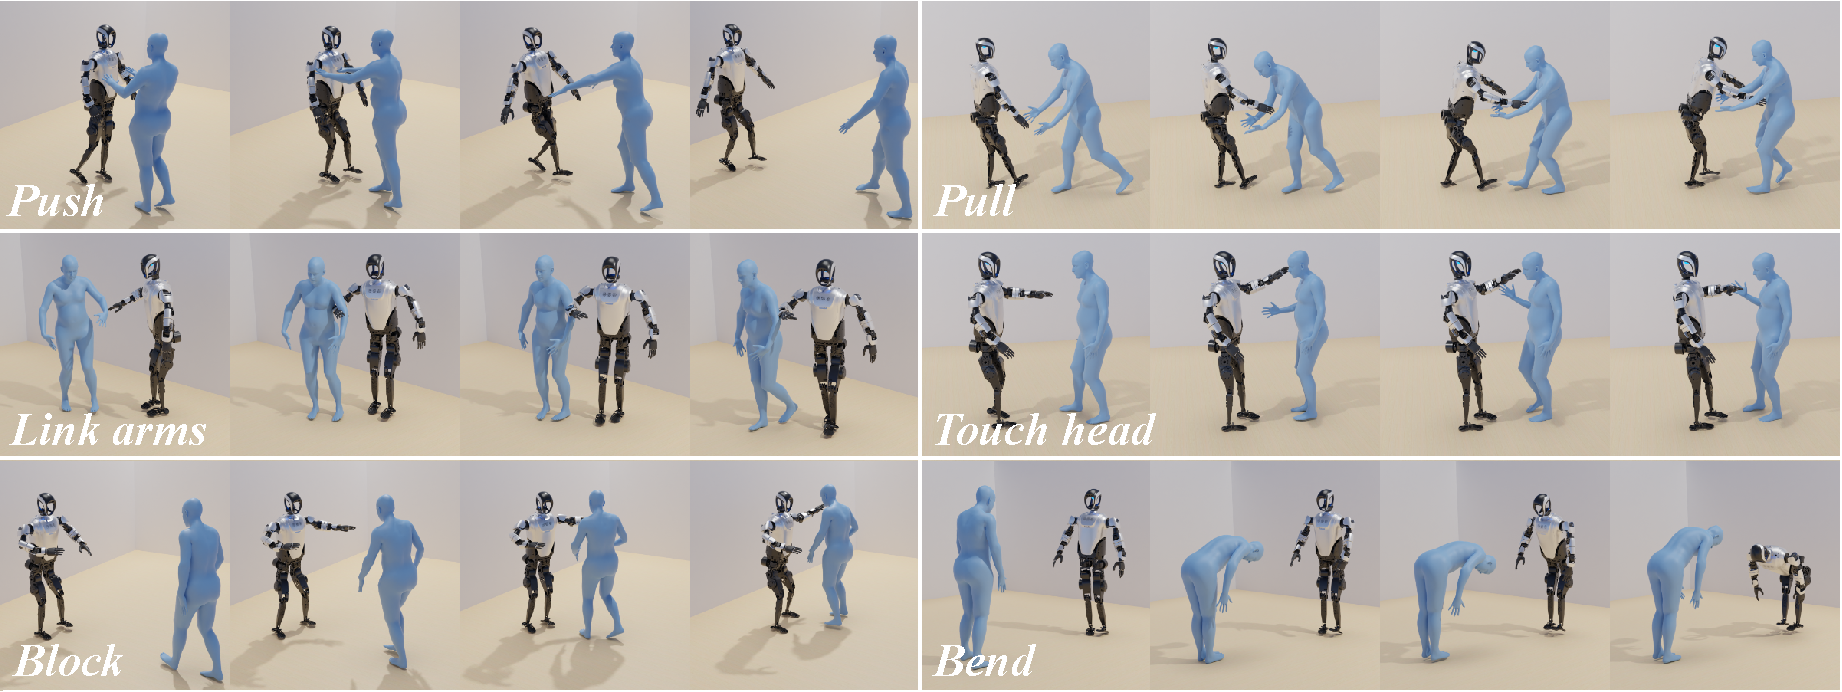
\includegraphics[width=1.0\linewidth]{images/vis-ours-new-1-v1-crop.pdf}
\end{figure*}
\begin{figure*}[h]
\centering
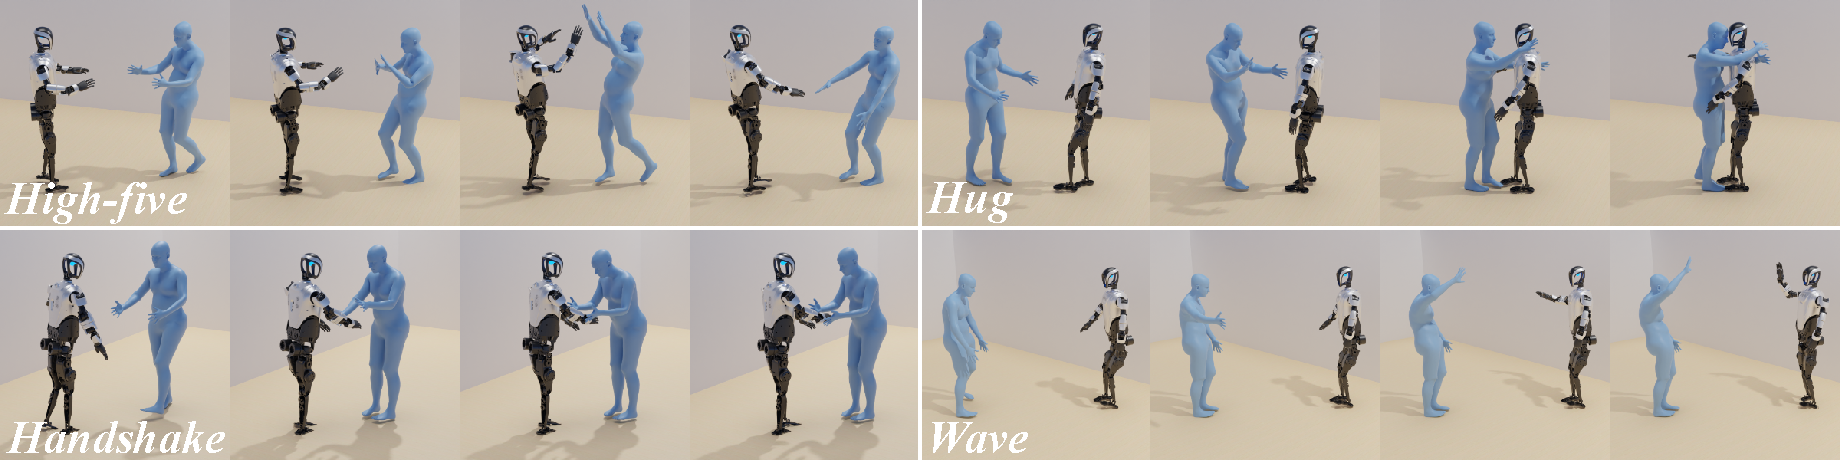
\includegraphics[width=1.0\linewidth]{images/vis-ours-new-0-v1-crop.pdf}
\vspace{-20px}
\caption{Visualizations of diverse human-robot interactions generated by our proposed Robotic Interaction Model. These sequences illustrate the model's capability to produce contextually appropriate and varied robot responses to dynamic human actions.}%, showcasing its effectiveness for enabling natural and engaging interactions.}%
\label{fig:visintermodel-ours}
\vspace{-5px}
\end{figure*}


\begin{figure*}[b]
\centering
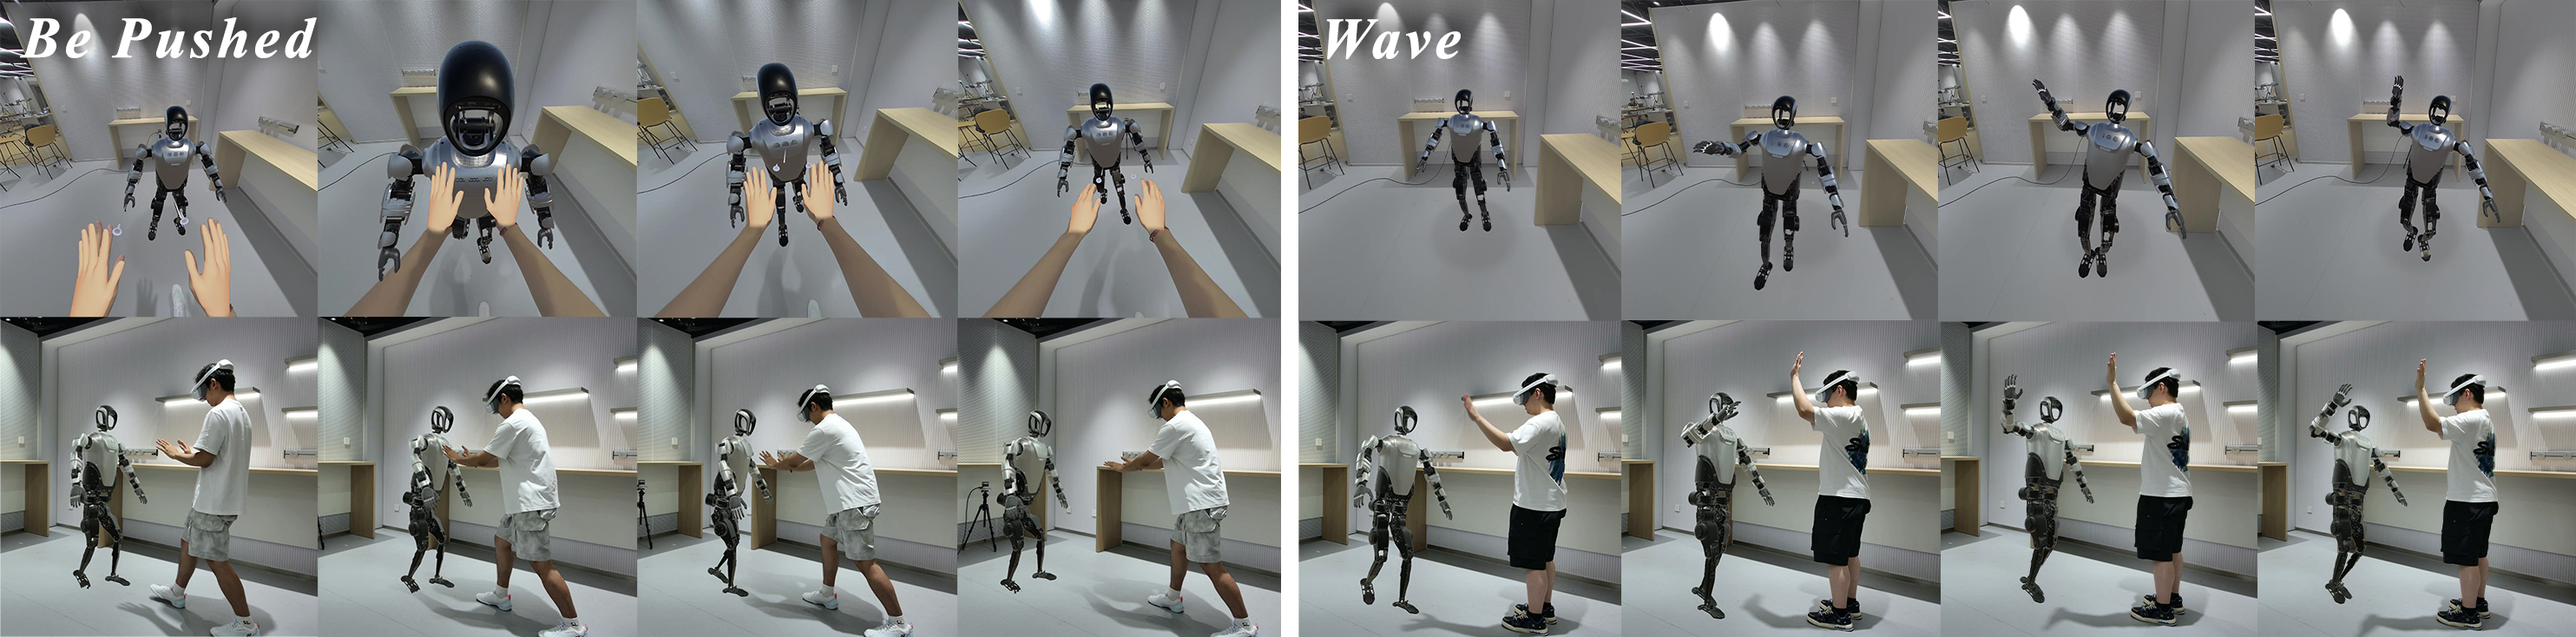
\includegraphics[width=1.0\linewidth]{images/interact.png}
\vspace{-20px}
\caption{The human-robot interactions presented in our system. Top: The first-person perspective visualized via the AR glasses. Bottom: The third-person perspective produced by fusing the captured human user in the physical environment and the rendered virtual robot.}
\label{fig:systeminter}
\end{figure*}

\begin{figure*}[h]
\centering
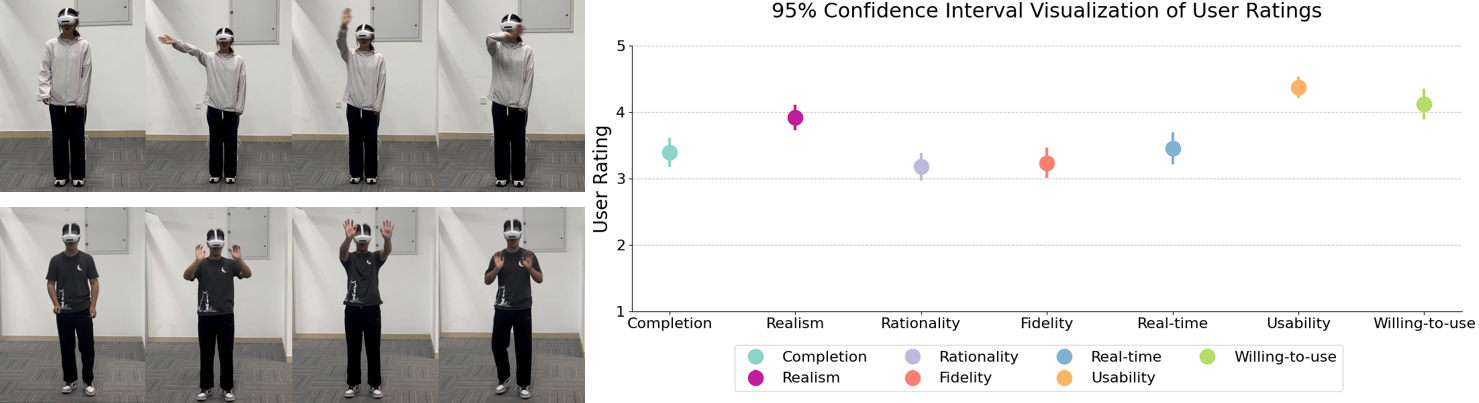
\includegraphics[width=1.0\linewidth]{images/reeeeeee.png}
\vspace{-20px}
\caption{Process and results of the user empirical test. Left: Participants interacting with virtual robots via our system. Right: The 95$\%$ confidence interval visualization of user ratings showing the mean and boundary of the confidence intervals. Here, 1 indicates "poor" and 5 indicates "excellent".}
\label{fig:userstudy}
\end{figure*}
\vspace{-20px}
\begin{figure*}[b]
\centering
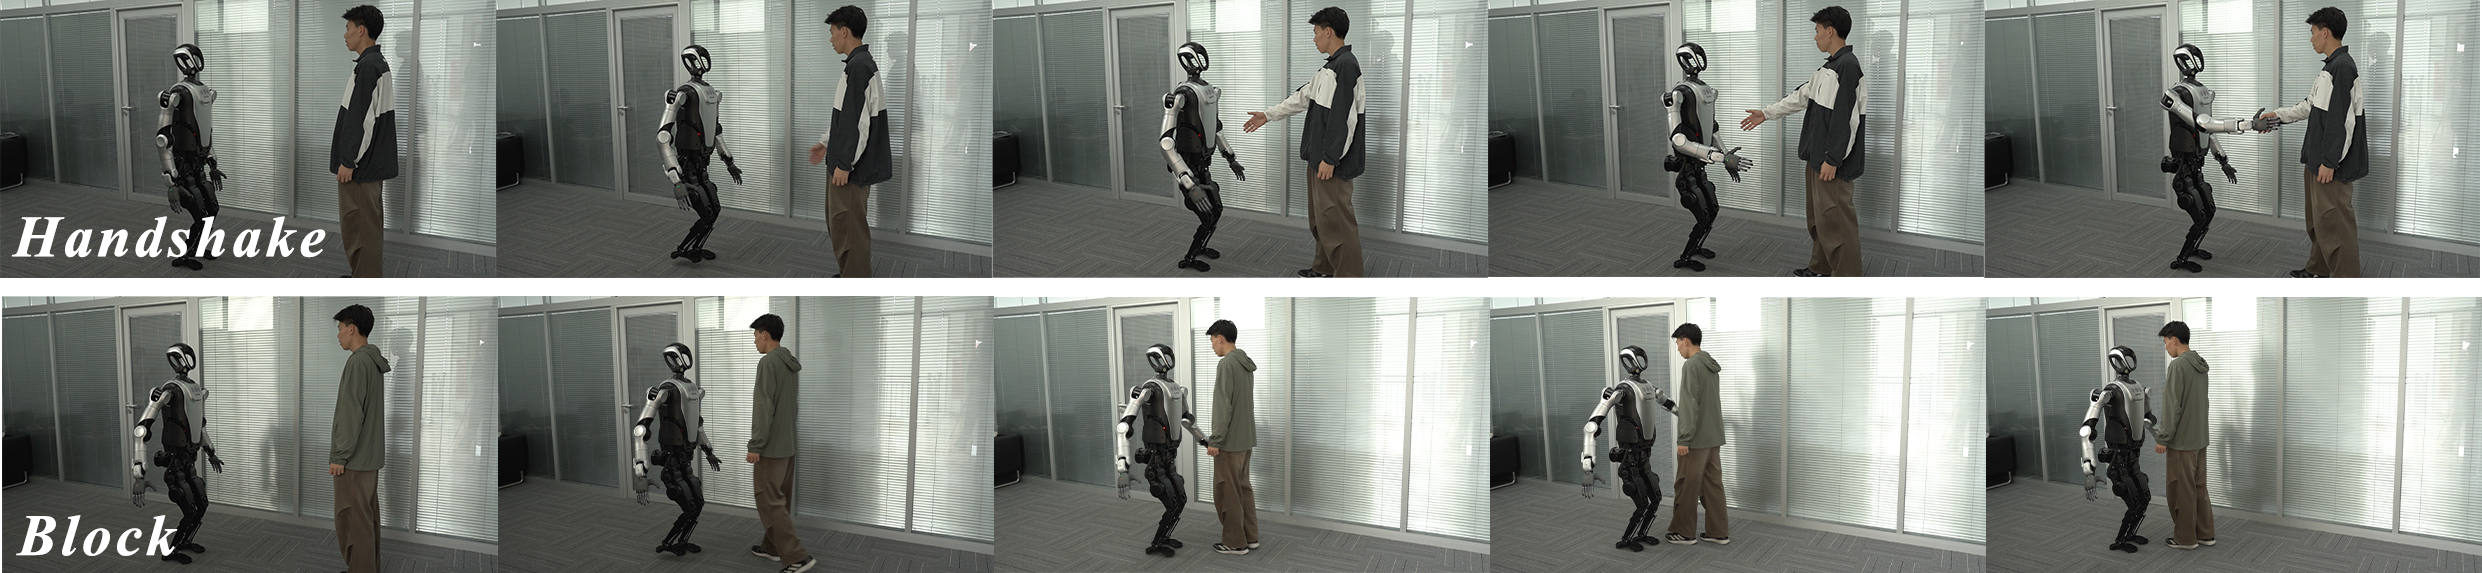
\includegraphics[width=1.0\linewidth]{images/physicalrobot.png}
\vspace{-20px}
\caption{A real LEJU Kuavo robot performing the robot movements generated by the robotic interaction model. Since the real robot exhibits a high consistency with the appearance of the virtual robot shown in our system, a human user can easily and smoothly interact with the real robot.}
\vspace{-20px}
\label{fig:realrobot}
\end{figure*}



\appendix


\end{document}
